\documentclass[11pt,letterpaper]{refart}

\usepackage{gitinfo2}
\usepackage{amsmath,mathtools}

\usepackage{hyperref}
\usepackage{cleveref}
\usepackage{caption}
\usepackage{subcaption}

\usepackage{microtype}
\usepackage[T1]{fontenc}

\usepackage{graphicx}
\usepackage{xcolor}
\usepackage{framed}
\usepackage{booktabs}
\usepackage{siunitx}  % Better kerning
\usepackage[section]{placeins}  % Figures can only float within its section

\usepackage{chngcntr}
\counterwithin{figure}{section}

\usepackage{tikz}
\tikzset{
    boximg/.style={remember picture,
                   ultra thick,
                   inner sep=0pt,
                   outer sep=0pt}
}

\def\itwoc{I{$\scriptstyle^2$}C\ }
\newcommand\symbolwithin[2]{%
{\mathmakebox[\widthof{\ensuremath{{}#2{}}}][c]{{#1}}}}

\title{DCB Design Verification Measurements}
\author{University of Maryland LHCb group}

\begin{document}
\maketitle
\hfill\small{\texttt{Rev:~\gitRel~(\gitAbbrevHash)}}
\tableofcontents
\listoffigures
\newpage


\section{Transient current}
We used a Gauss probe connected to an oscilloscope to measure current.
The probe was warped around the cable which was connected to the positive end of
the \SI{1.5}{\volt} PSU.

All the measurements below assume a conversion factor of \SI{1}{\ampere/\volt}.
DCB S/N pilot 007, 008 were used for measurements.

\begin{figure}[ht]
    \centering
    \begin{subfigure}{0.8\linewidth}
    \begin{tikzpicture}[boximg]
        \node [anchor=south west] (main) {
            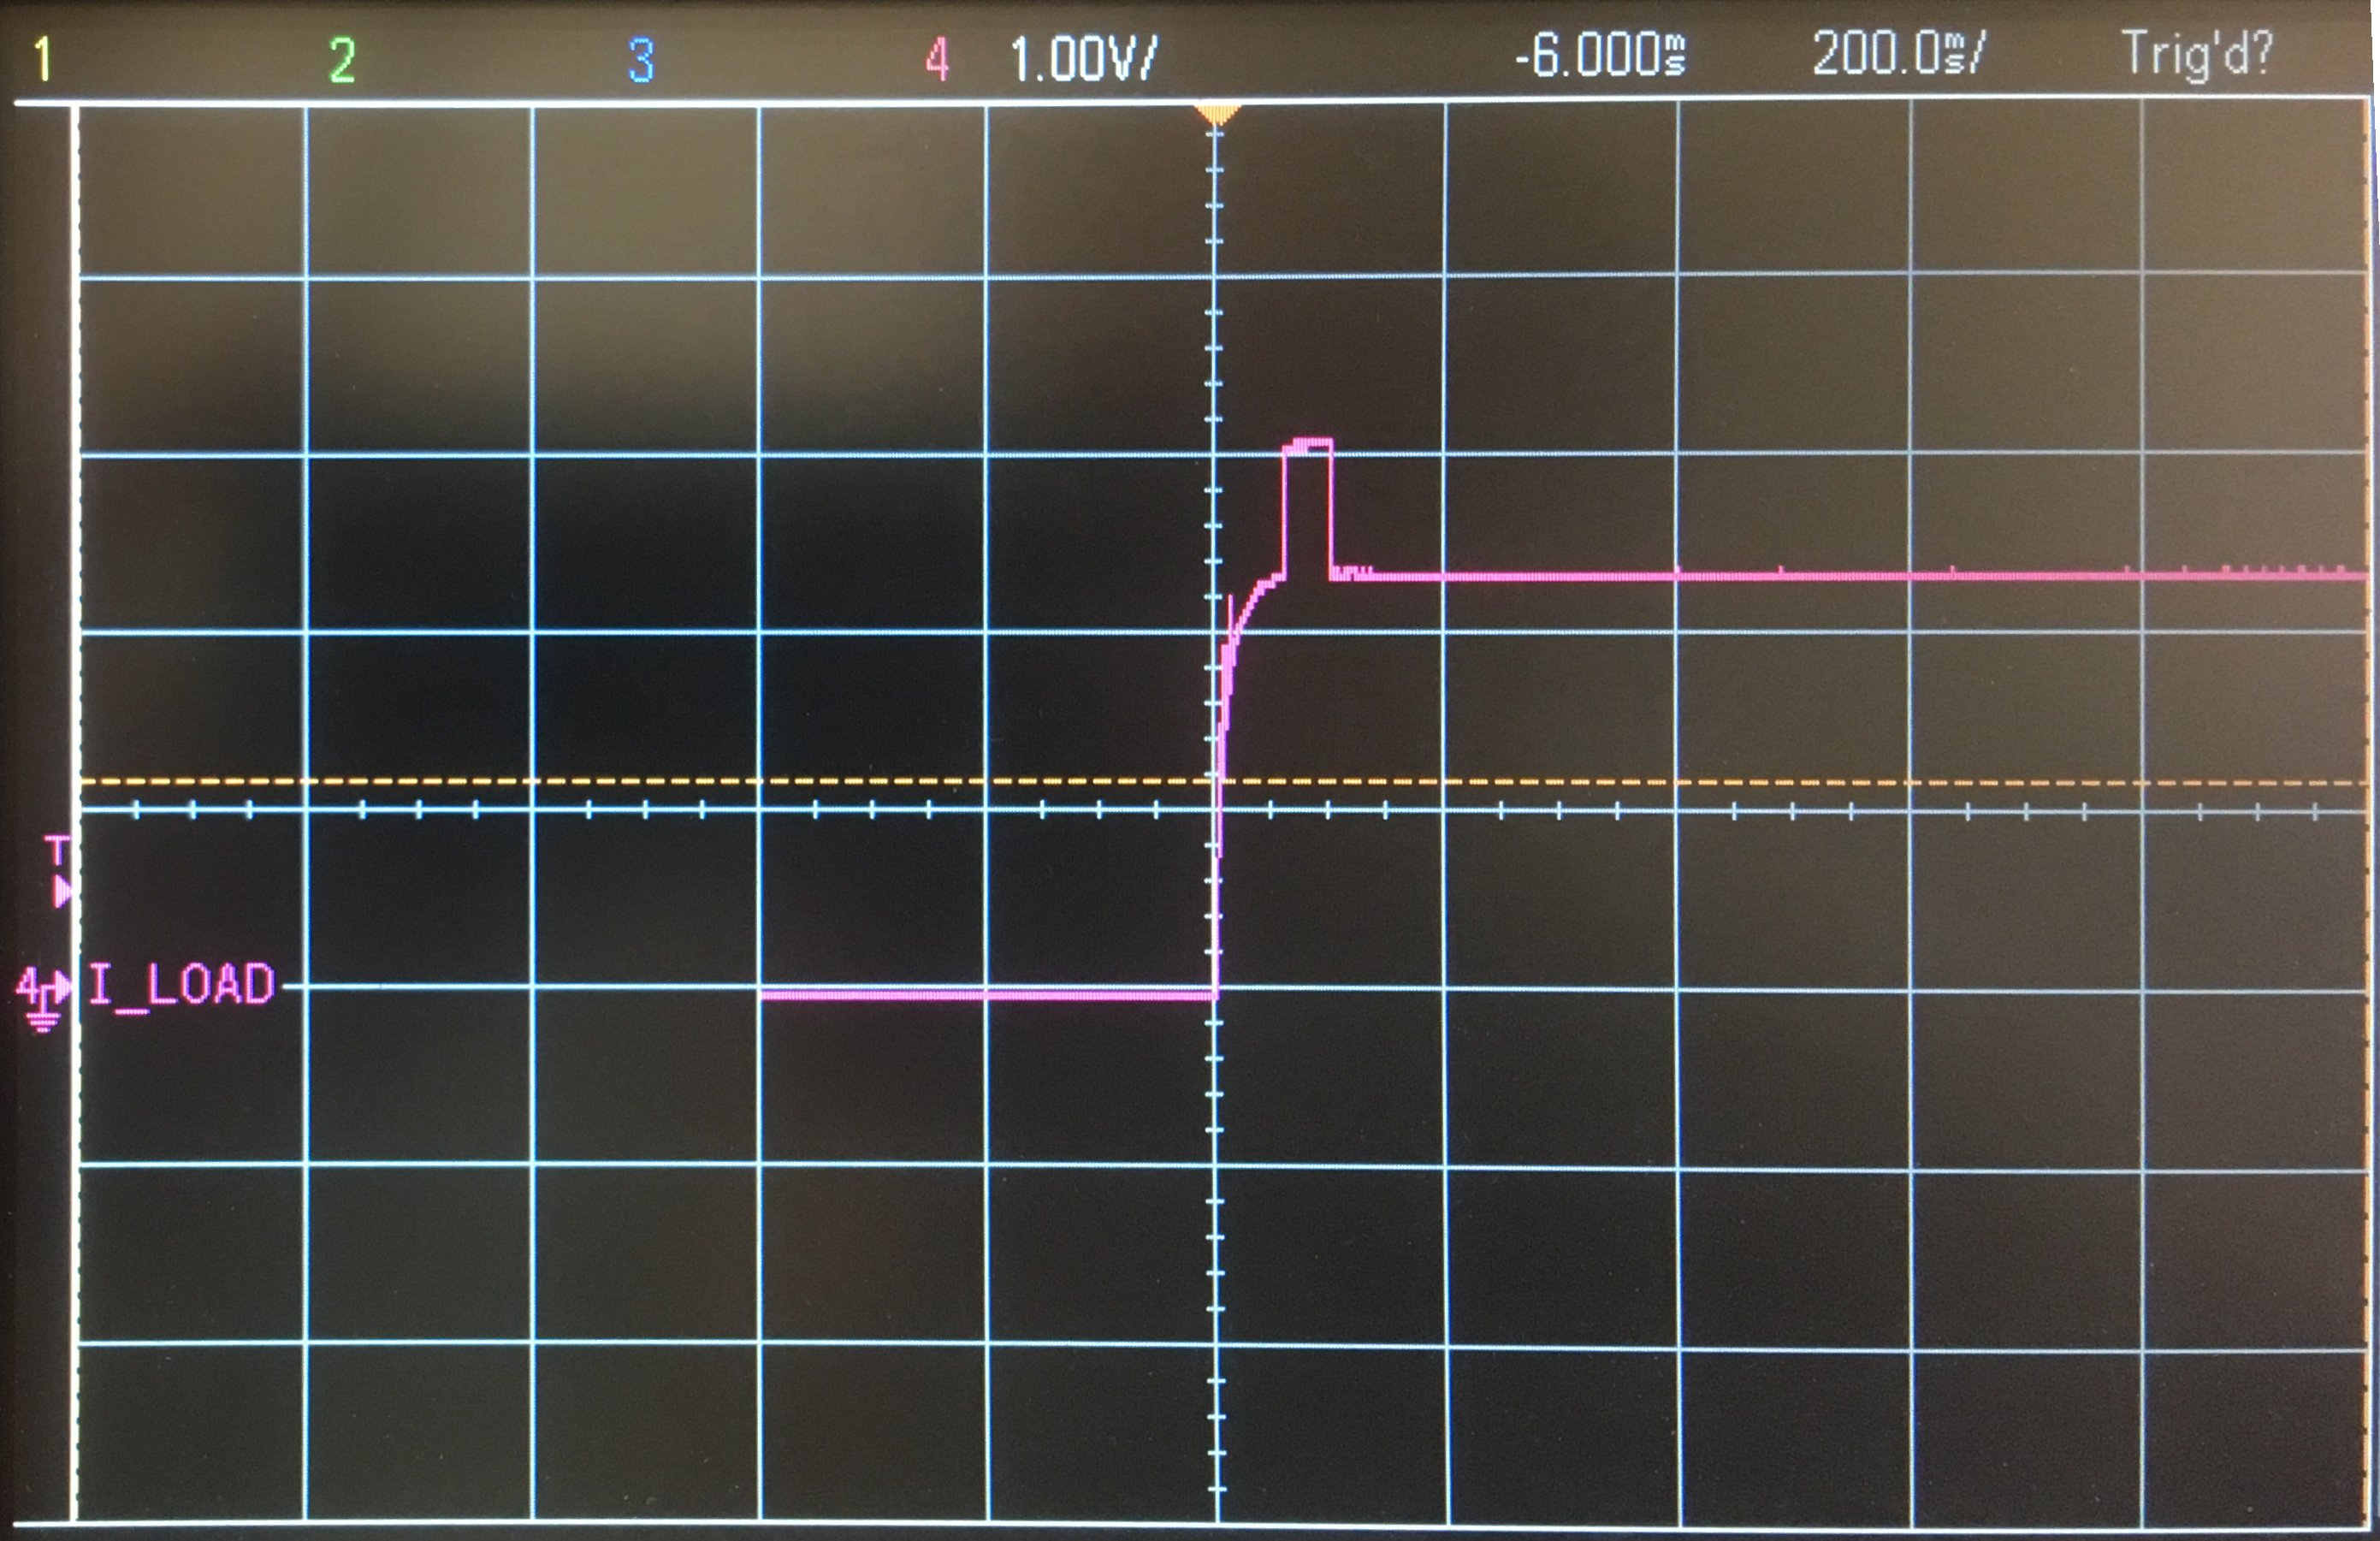
\includegraphics[width=\linewidth]
                {./res/current_transient/power_on.jpg}
        };
        \begin{scope}[x=(main.south east),y=(main.north west)]
            \node [draw,red,minimum height=5em, minimum width=2em] (zoombox1)
                at (0.5,0.5) {};
        \end{scope}
    \end{tikzpicture}
    \caption{}
    \end{subfigure}
    %
    \\[0.5\baselineskip]
    %
    \begin{subfigure}{0.5\linewidth}
    \begin{tikzpicture}[boximg,red]
        \node (zoom1) {
            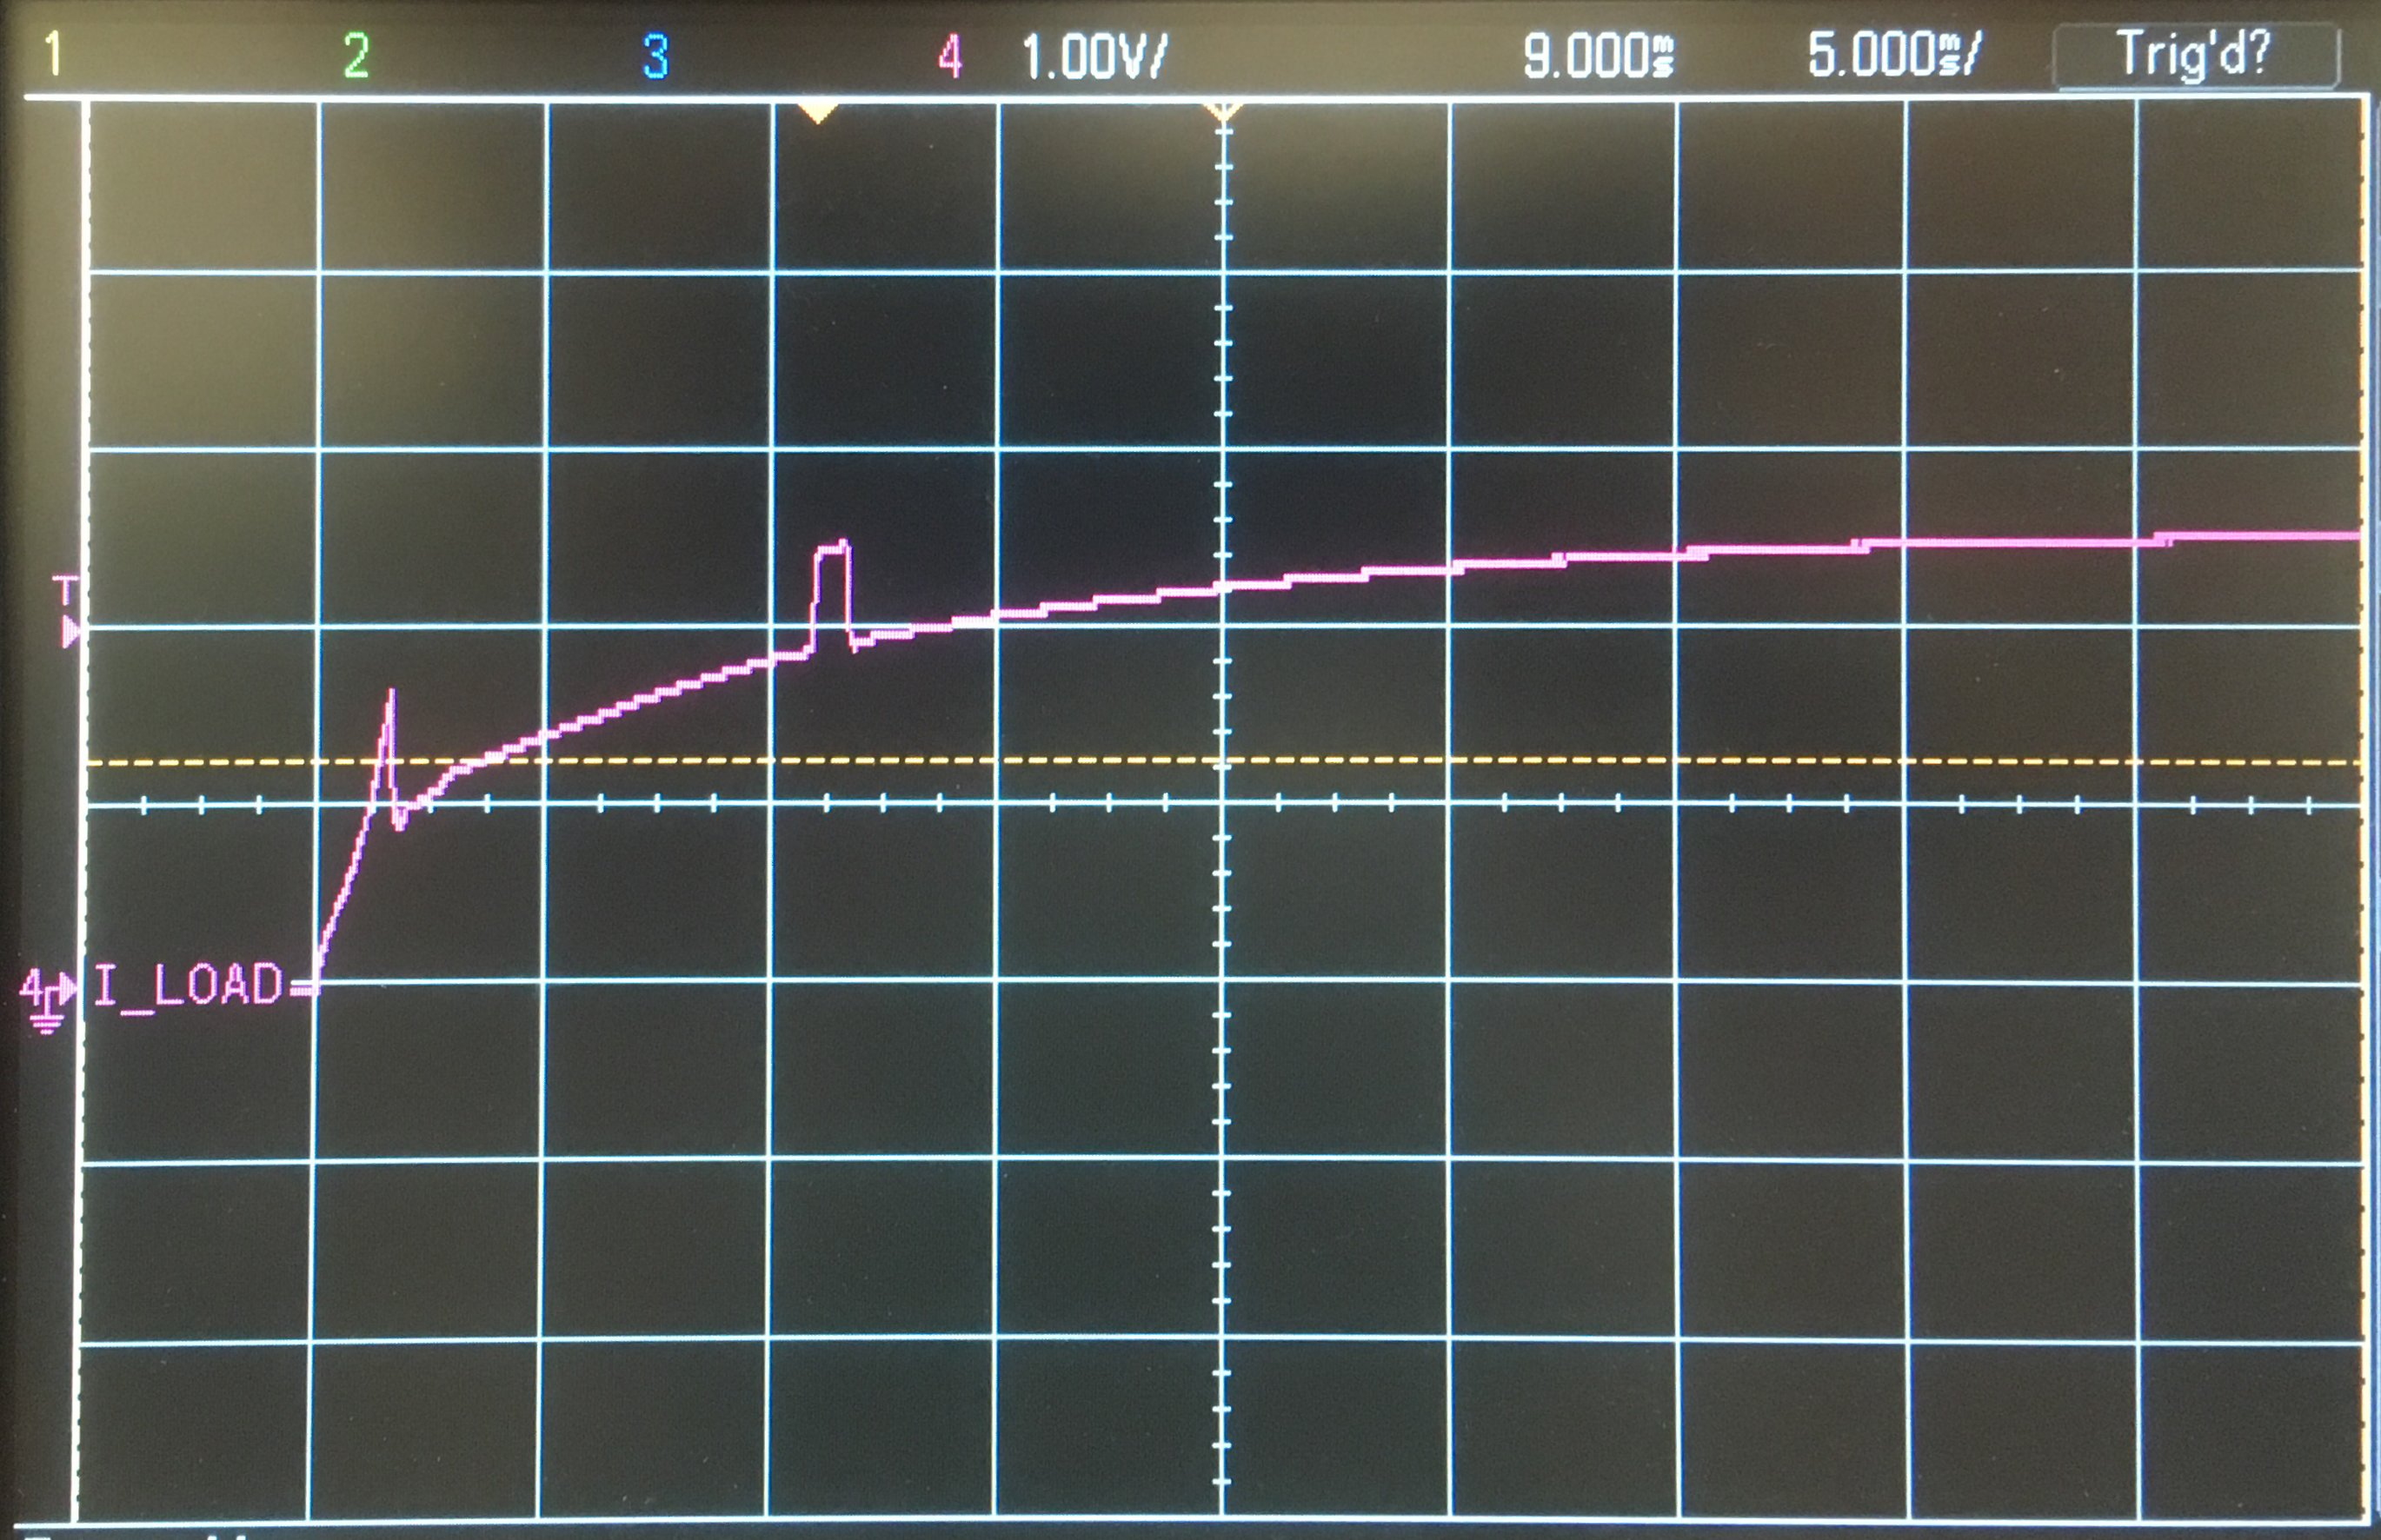
\includegraphics[width=\linewidth]
                {./res/current_transient/power_on-zoom.jpg}
        };
        \draw (zoom1.south west) rectangle (zoom1.north east);
    \end{tikzpicture}
    \caption{}
    \end{subfigure}
    %\begin{tikzpicture}[overlay,boximg]
        %\draw (zoom1) -- (zoombox1);
    %\end{tikzpicture}
    \caption[Power on transient current]{
        Power on transient current. Measured on 007.
    }
\end{figure}

\begin{figure}[ht]
    \centering
    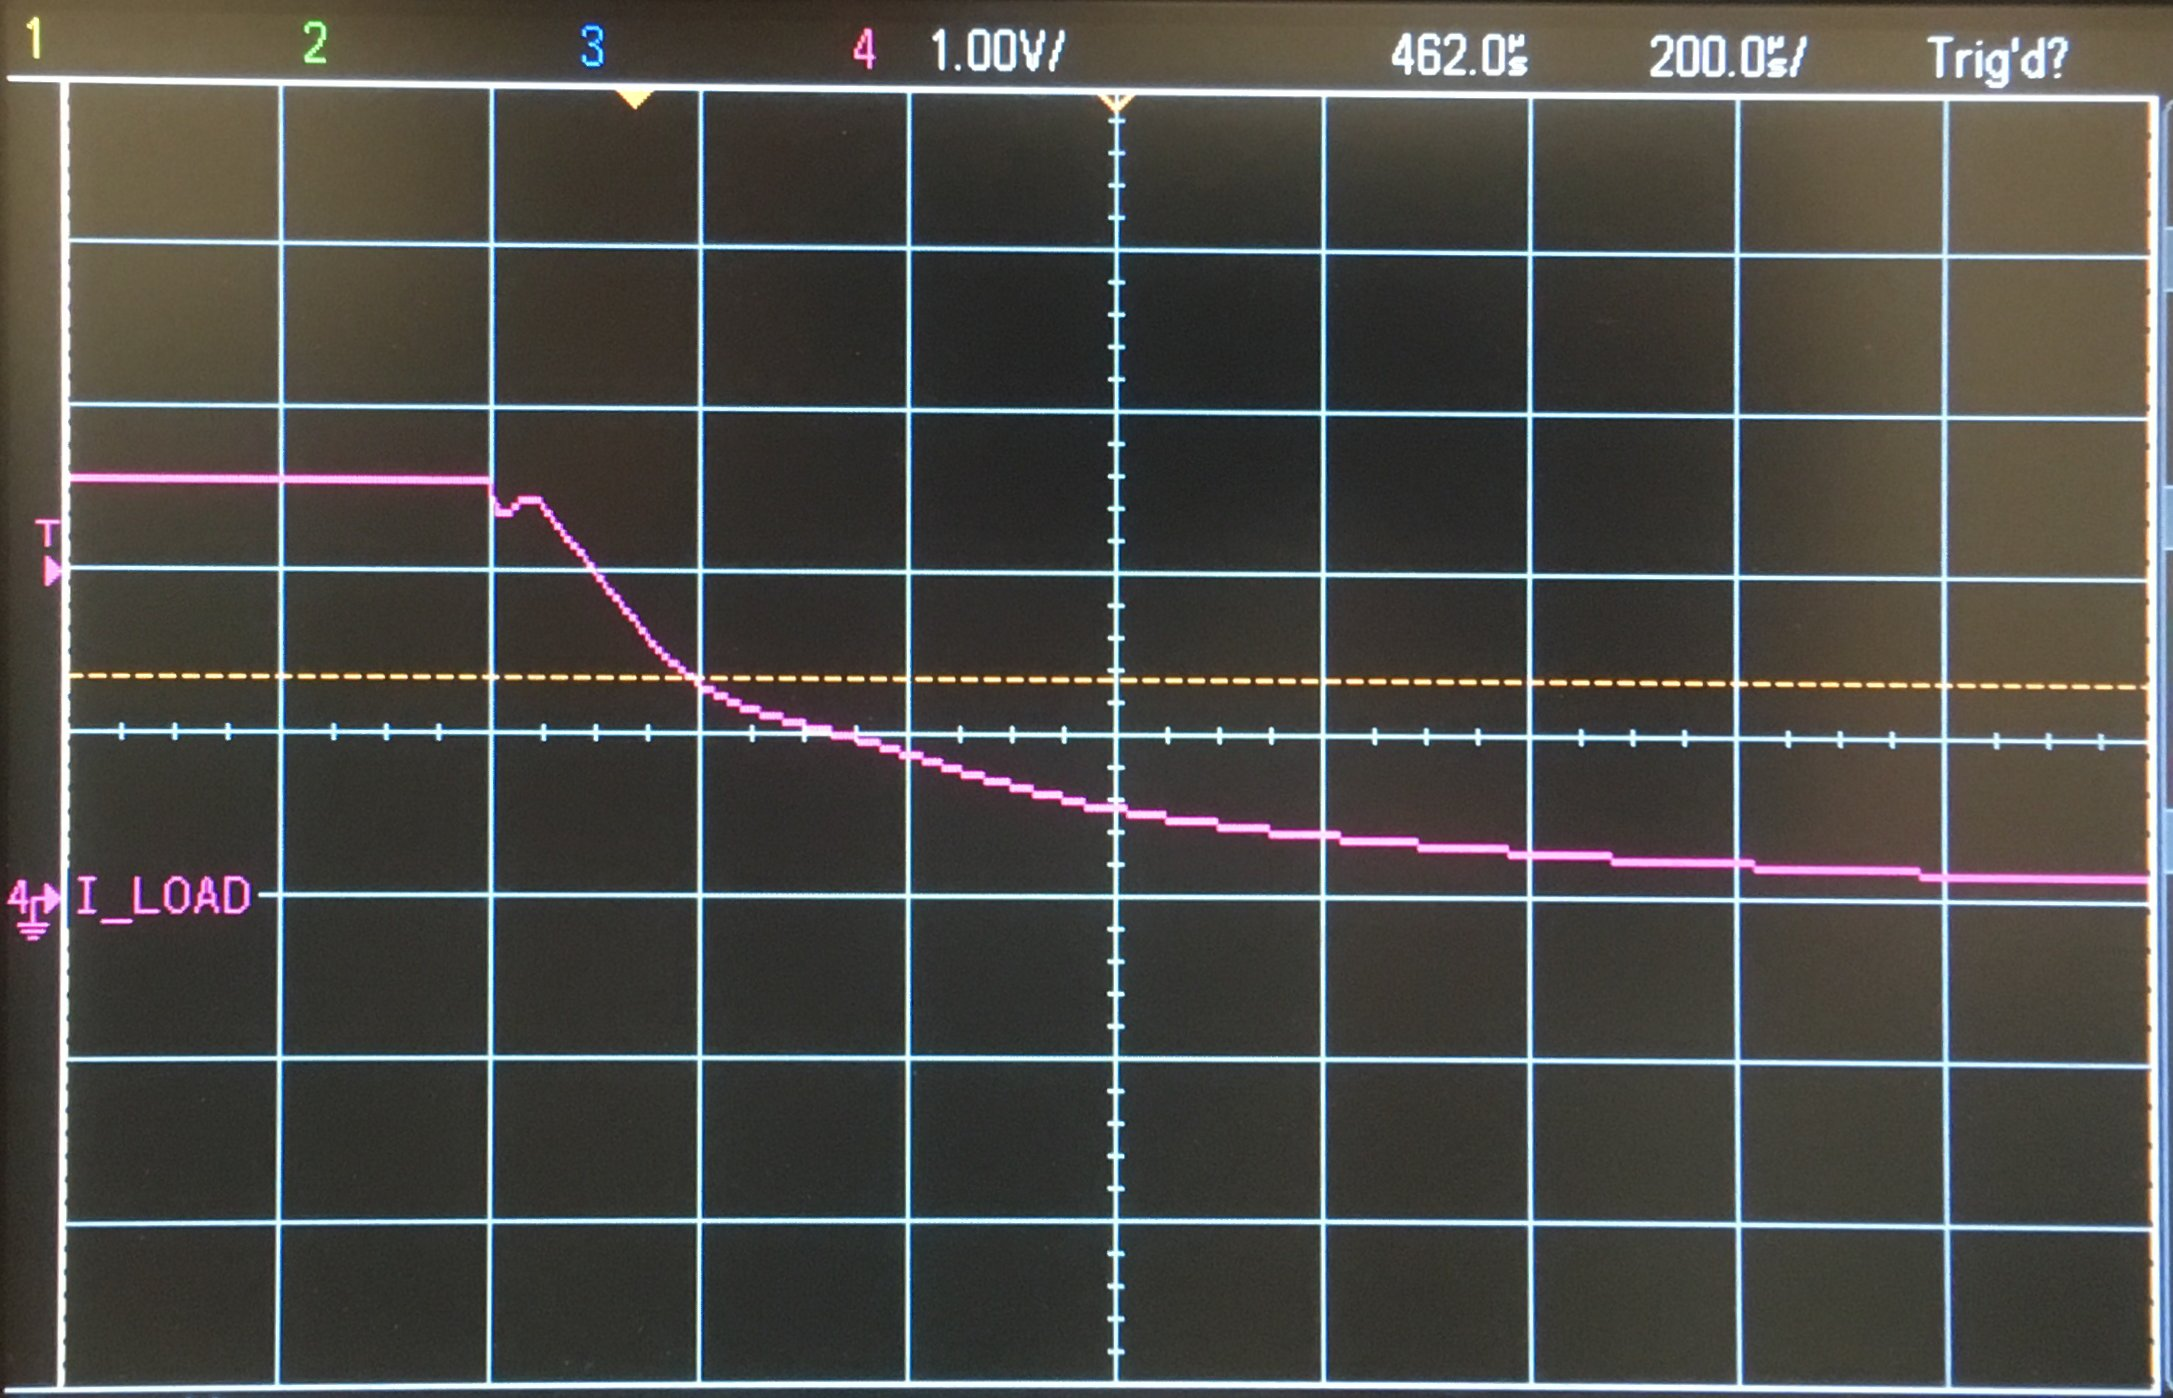
\includegraphics[width=0.8\linewidth]{./res/current_transient/power_off.jpg}
    \caption[Power off transient current]{
        Power off transient current. Measured on 007.
    }
\end{figure}

\begin{figure}[ht]
    \centering
    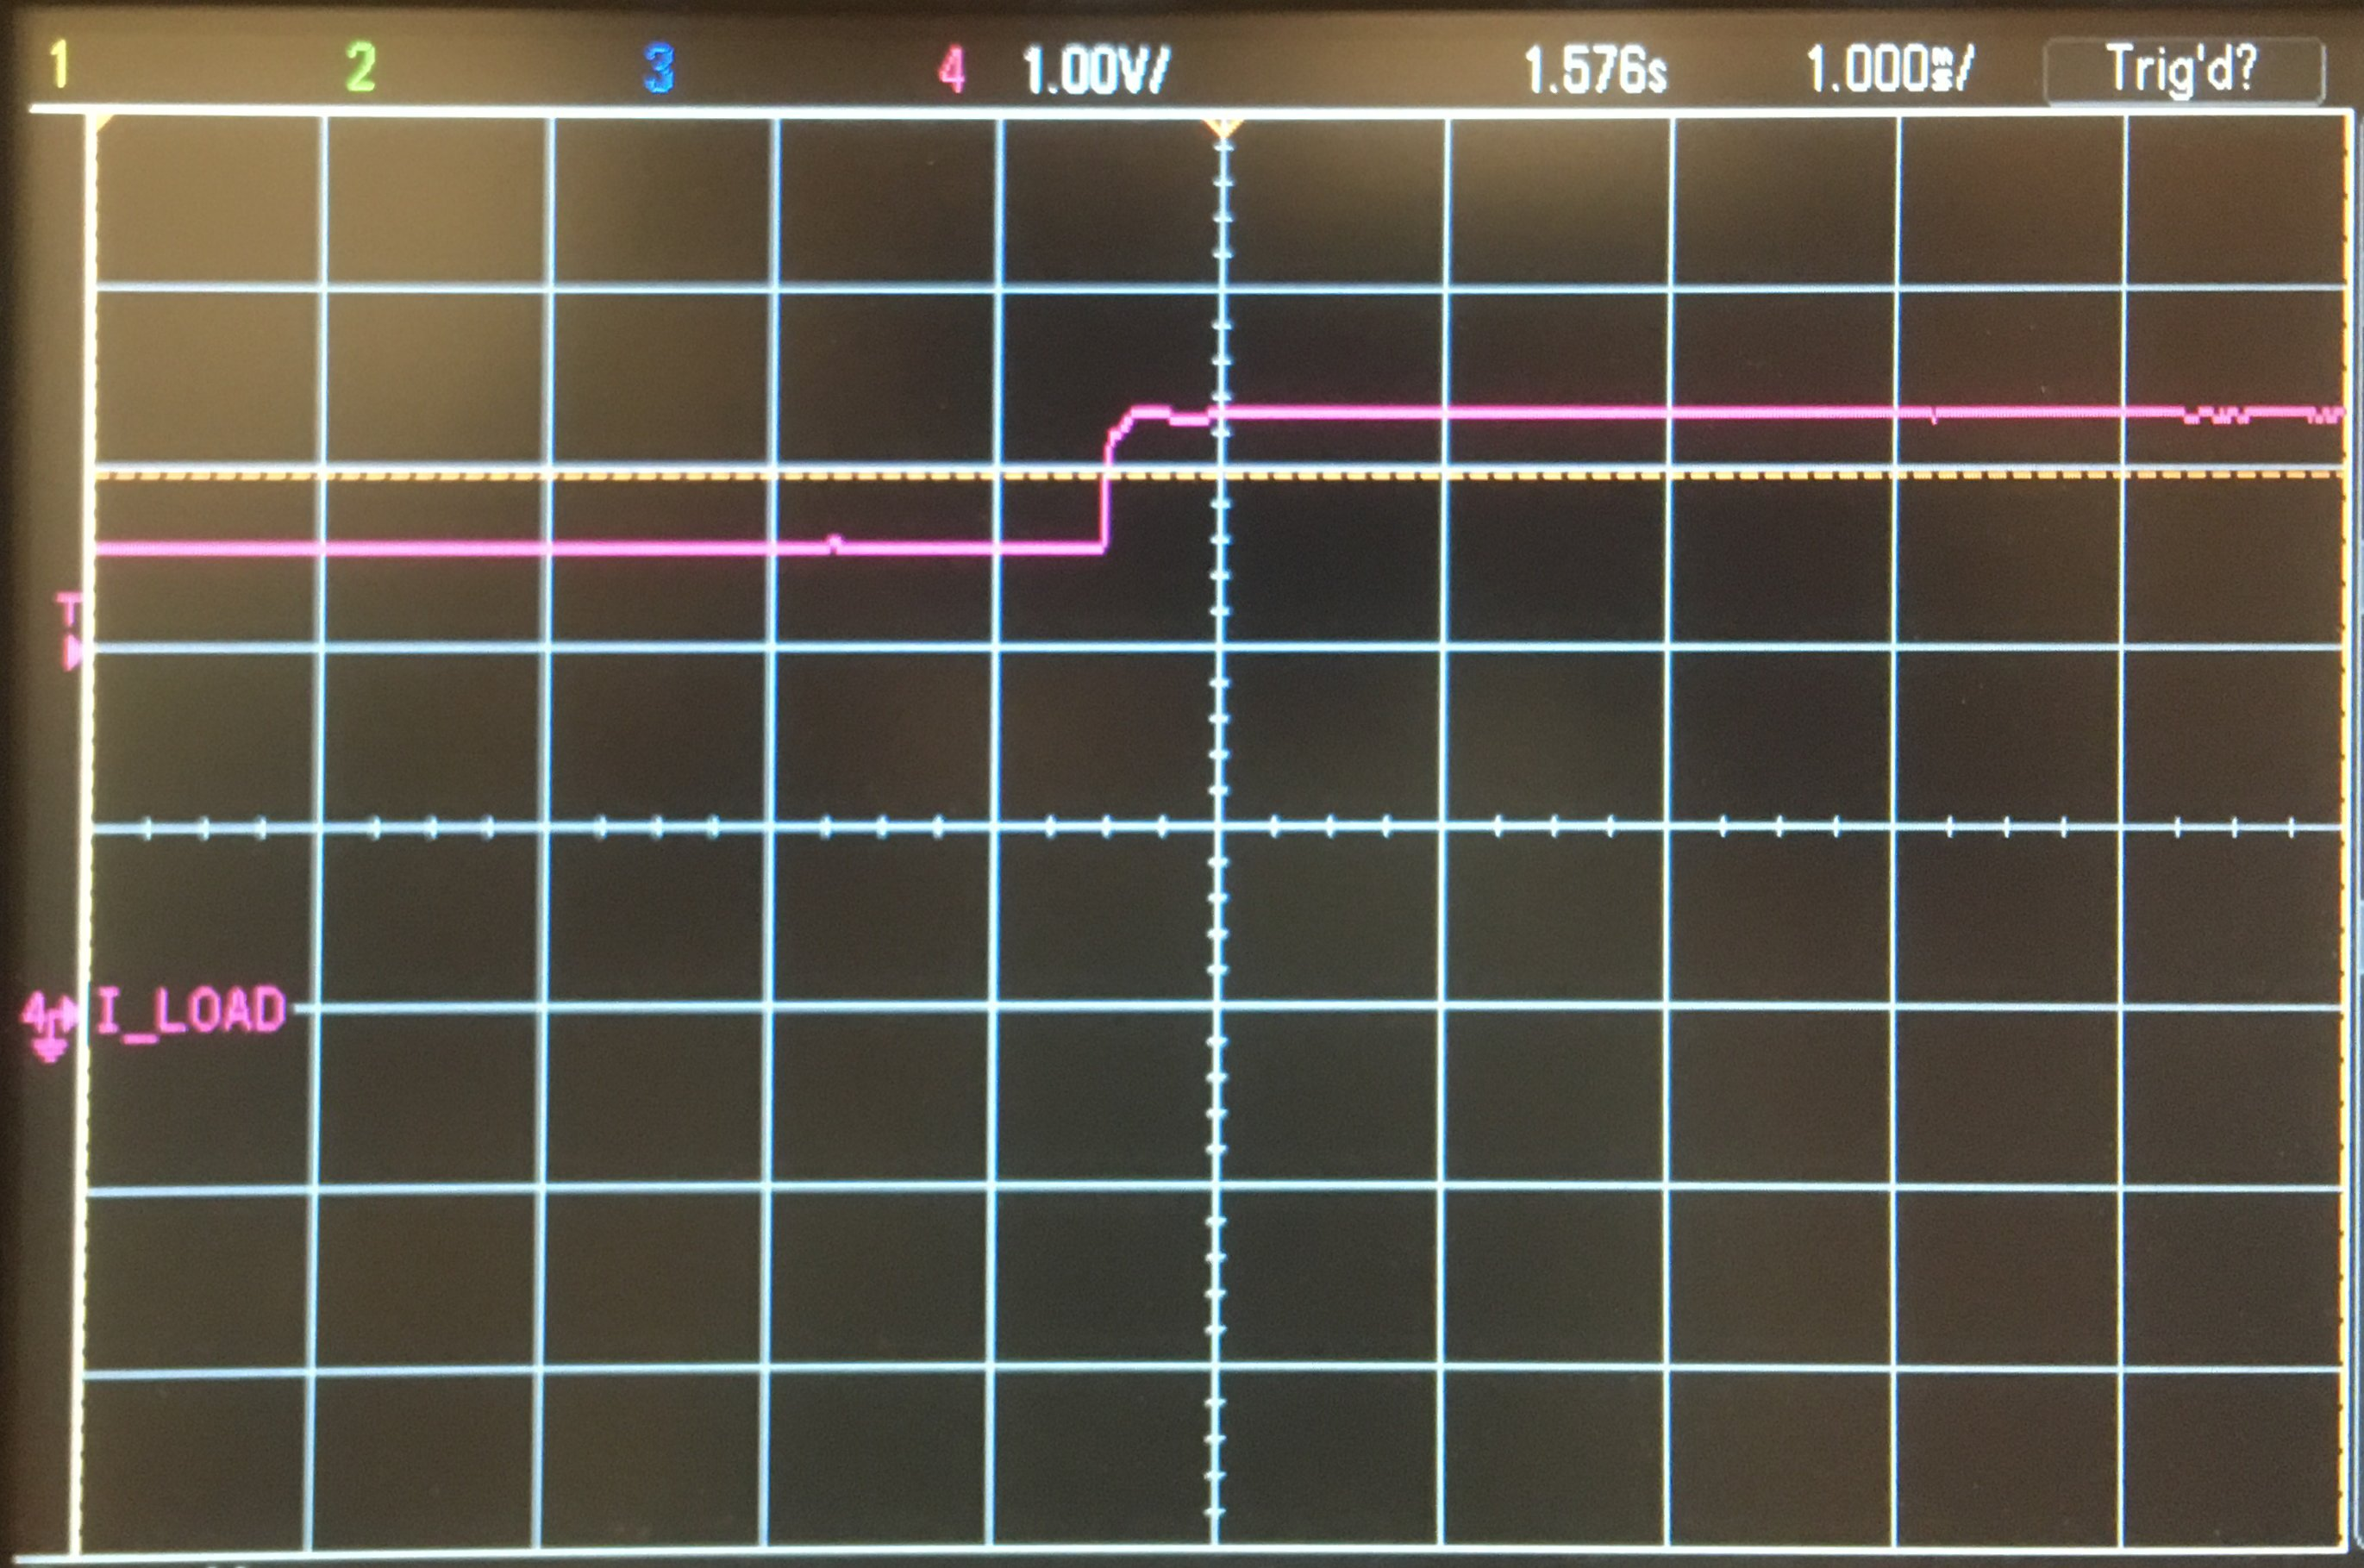
\includegraphics[width=0.8\linewidth]
        {./res/current_transient/program_master.jpg}
    \caption[Program master GBTx transient current]{
        Program master GBTx (via \itwoc) transient current.
        Measured on 007.
    }
\end{figure}

\begin{figure}[ht]
    \centering
    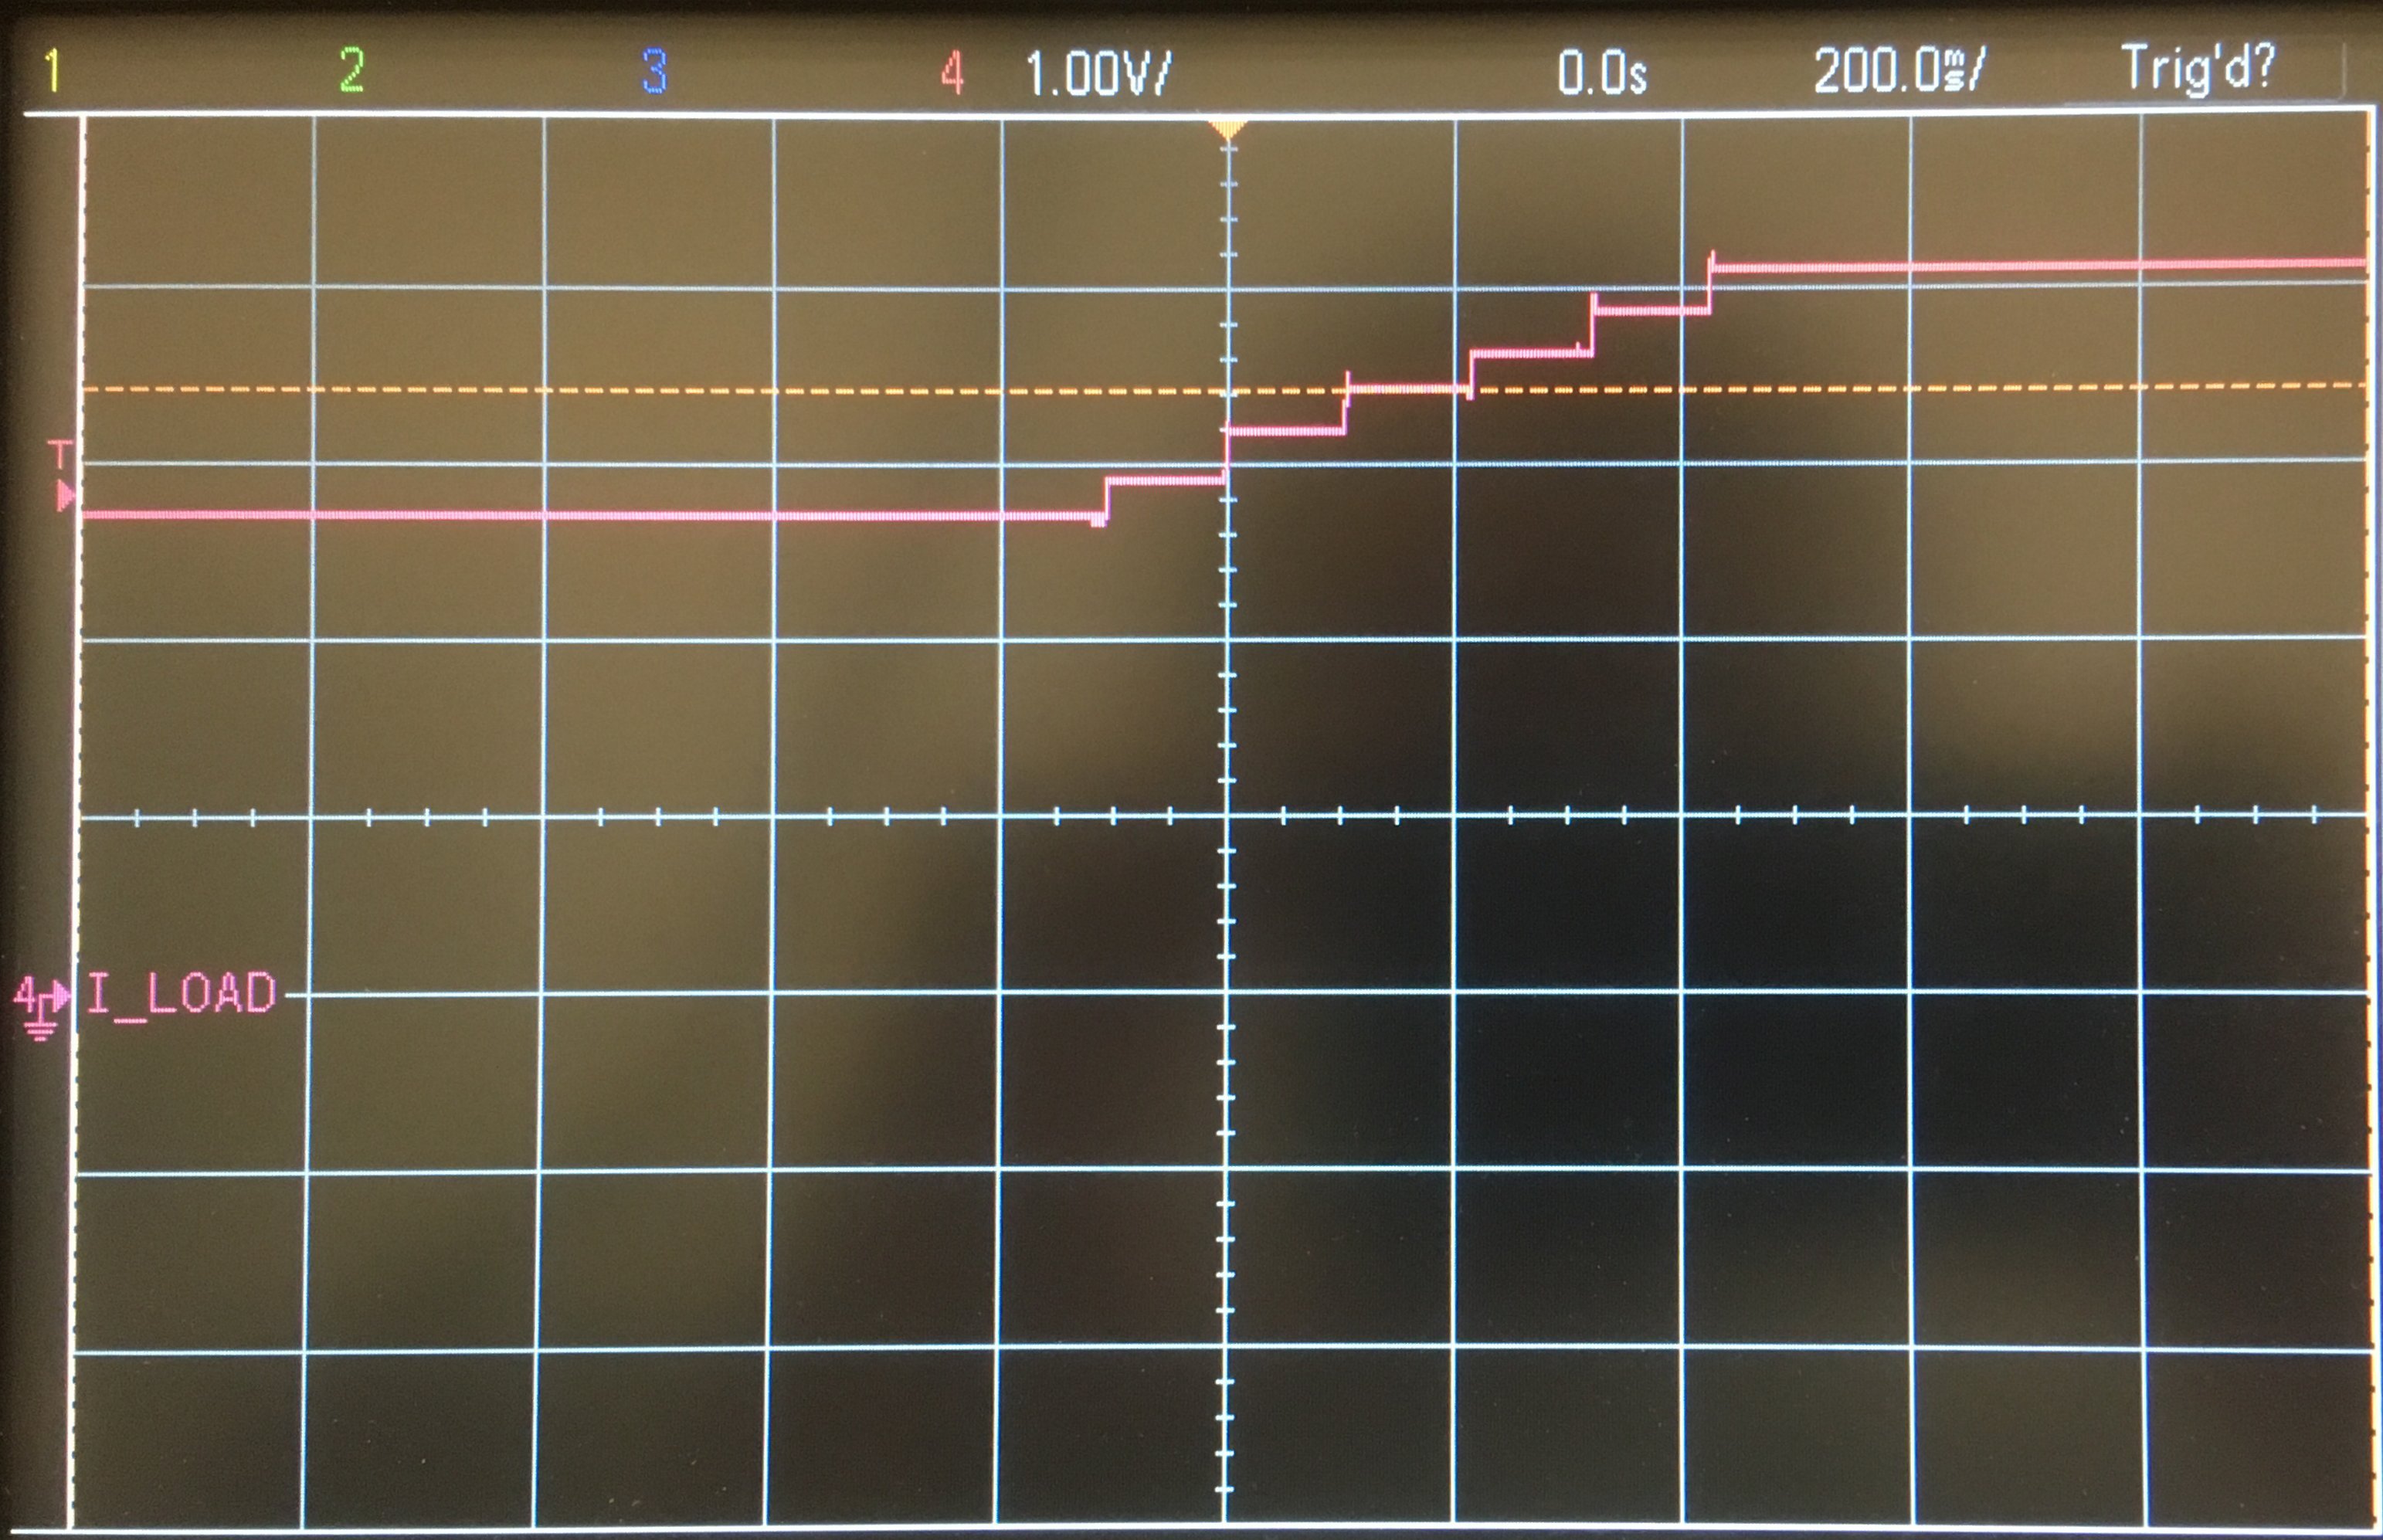
\includegraphics[width=0.8\linewidth]
        {./res/current_transient/program_data.jpg}
    \caption[Program data GBTxs transient current]{
        Program all 6 data GBTxs (via GBT-IC) transient current.
        The programmer on MiniDAQ is written in a way such that these data GBTxs
        are programmed one by one.
        Measured on 007.
    }
\end{figure}

\begin{figure}[ht]
    \centering
    \begin{subfigure}{0.8\linewidth}
    \begin{tikzpicture}[boximg]
        \node [anchor=south west] (main) {
            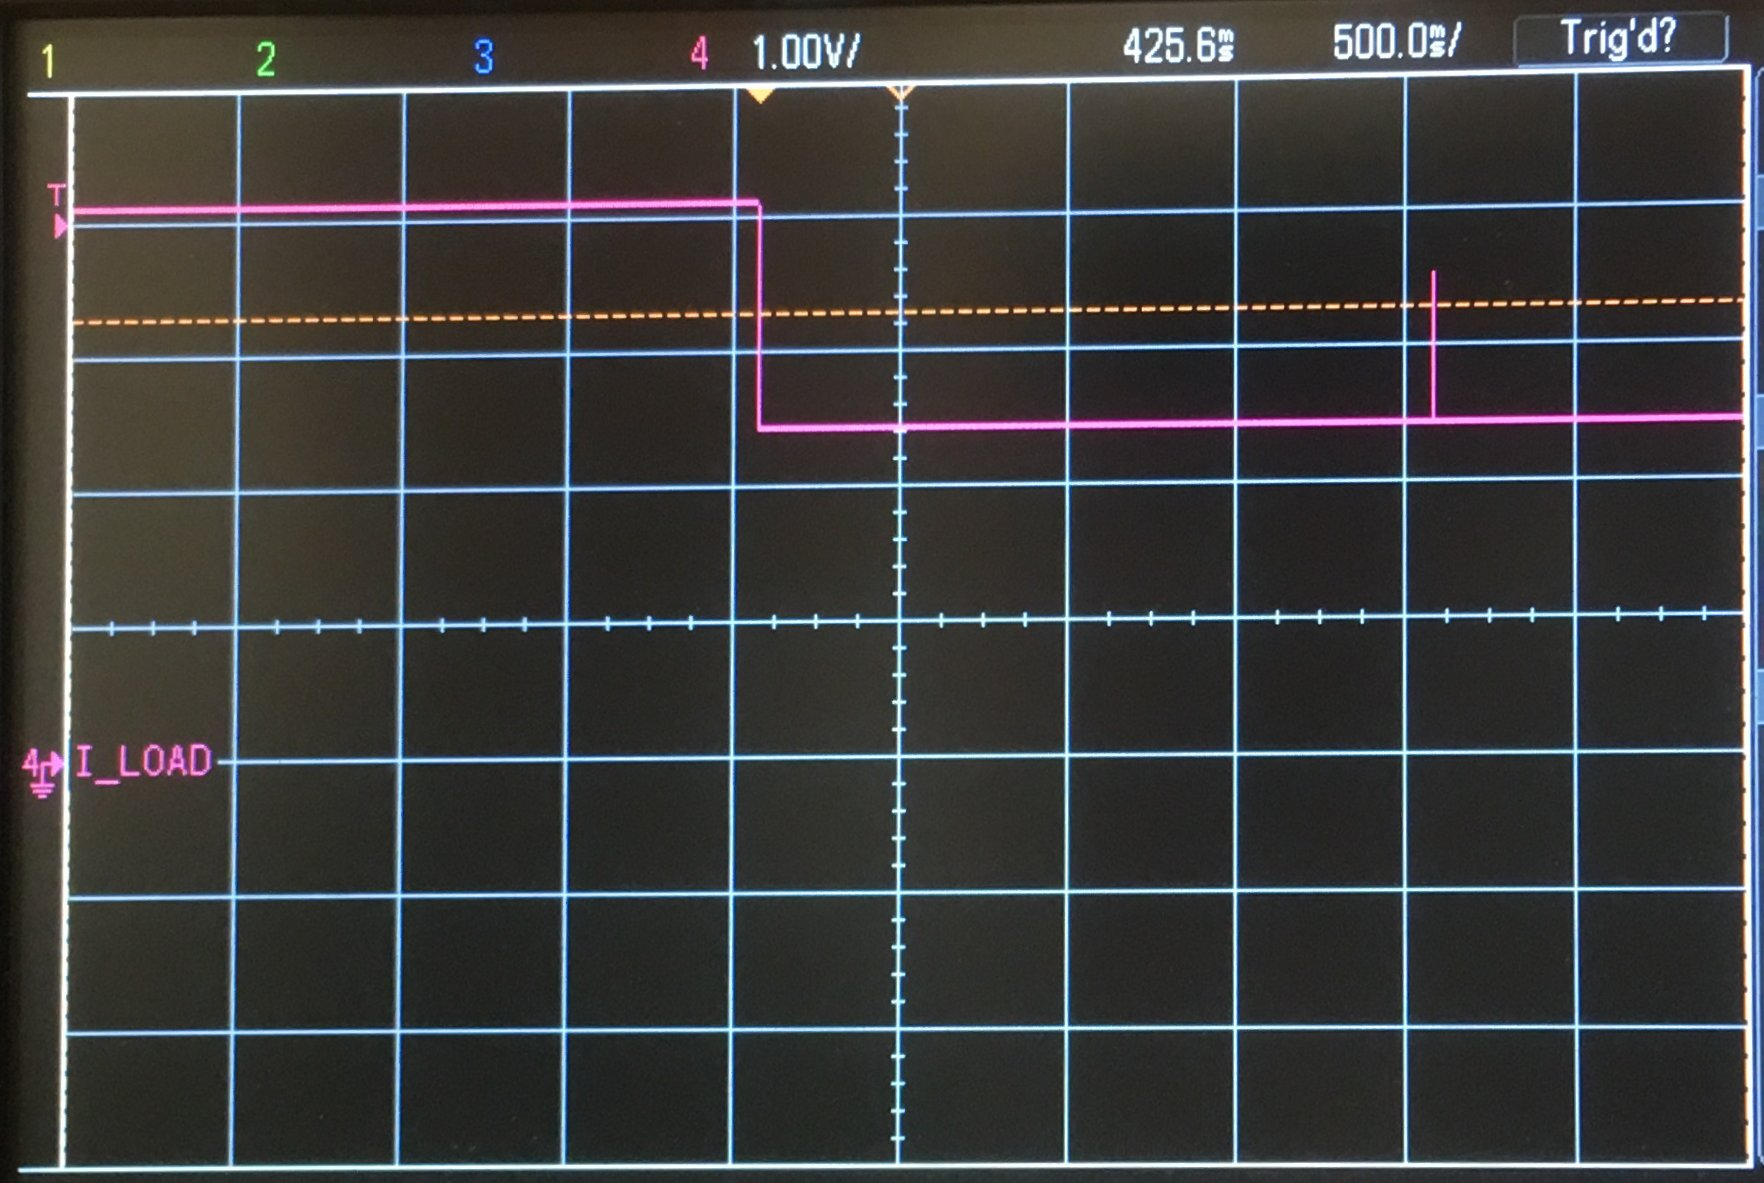
\includegraphics[width=\linewidth]
            {./res/current_transient/loss_of_lock.jpg}
        };
        \begin{scope}[x=(main.south east),y=(main.north west)]
            \node [draw,red,minimum height=4.5em, minimum width=1.5em]
                (zoombox1) at (0.42,0.72) {};
            \node [draw,green,minimum height=3.5em, minimum width=1.5em]
                (zoombox2) at (0.81,0.7) {};
        \end{scope}
    \end{tikzpicture}
    \caption{}
    \end{subfigure}
    %
    \\[0.5\baselineskip]
    %
    \begin{subfigure}{0.38\linewidth}
    \begin{tikzpicture}[boximg,red]
        \node (zoom1) {
            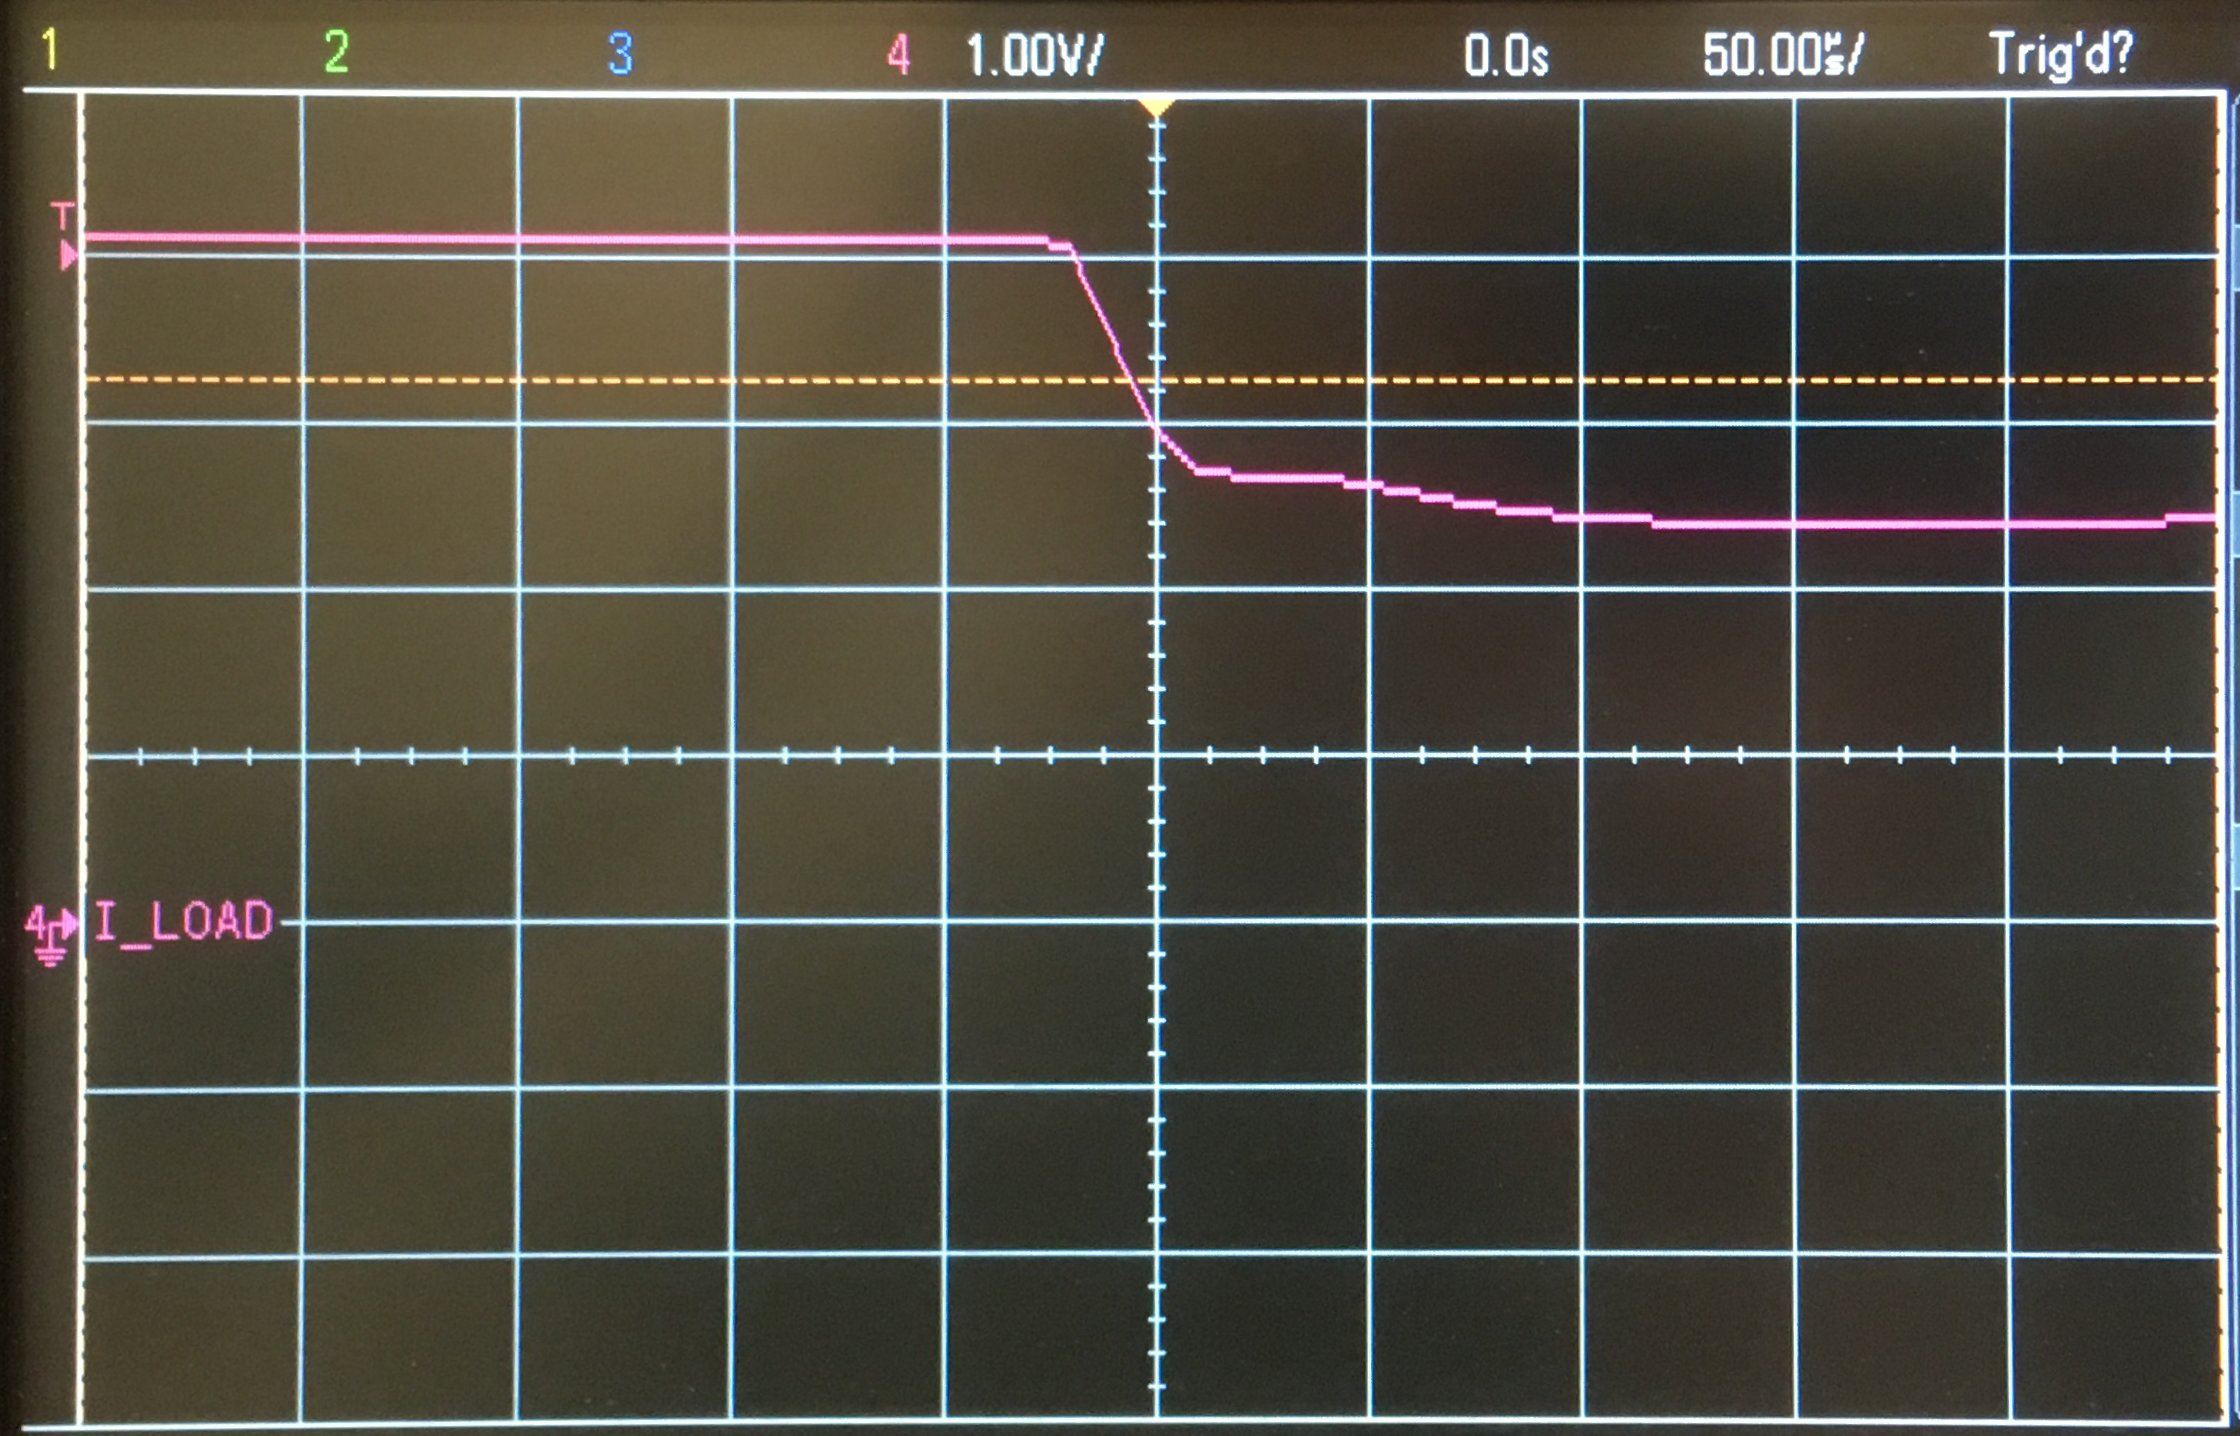
\includegraphics[width=\linewidth]
                {./res/current_transient/loss_of_lock-zoom1.jpg}
        };
        \draw (zoom1.south west) rectangle (zoom1.north east);
    \end{tikzpicture}
    \caption{}
    \end{subfigure}
    %
    \hspace{0.02\linewidth}
    %
    \begin{subfigure}{0.38\linewidth}
    \begin{tikzpicture}[boximg,green]
        \node  (zoom2) {
            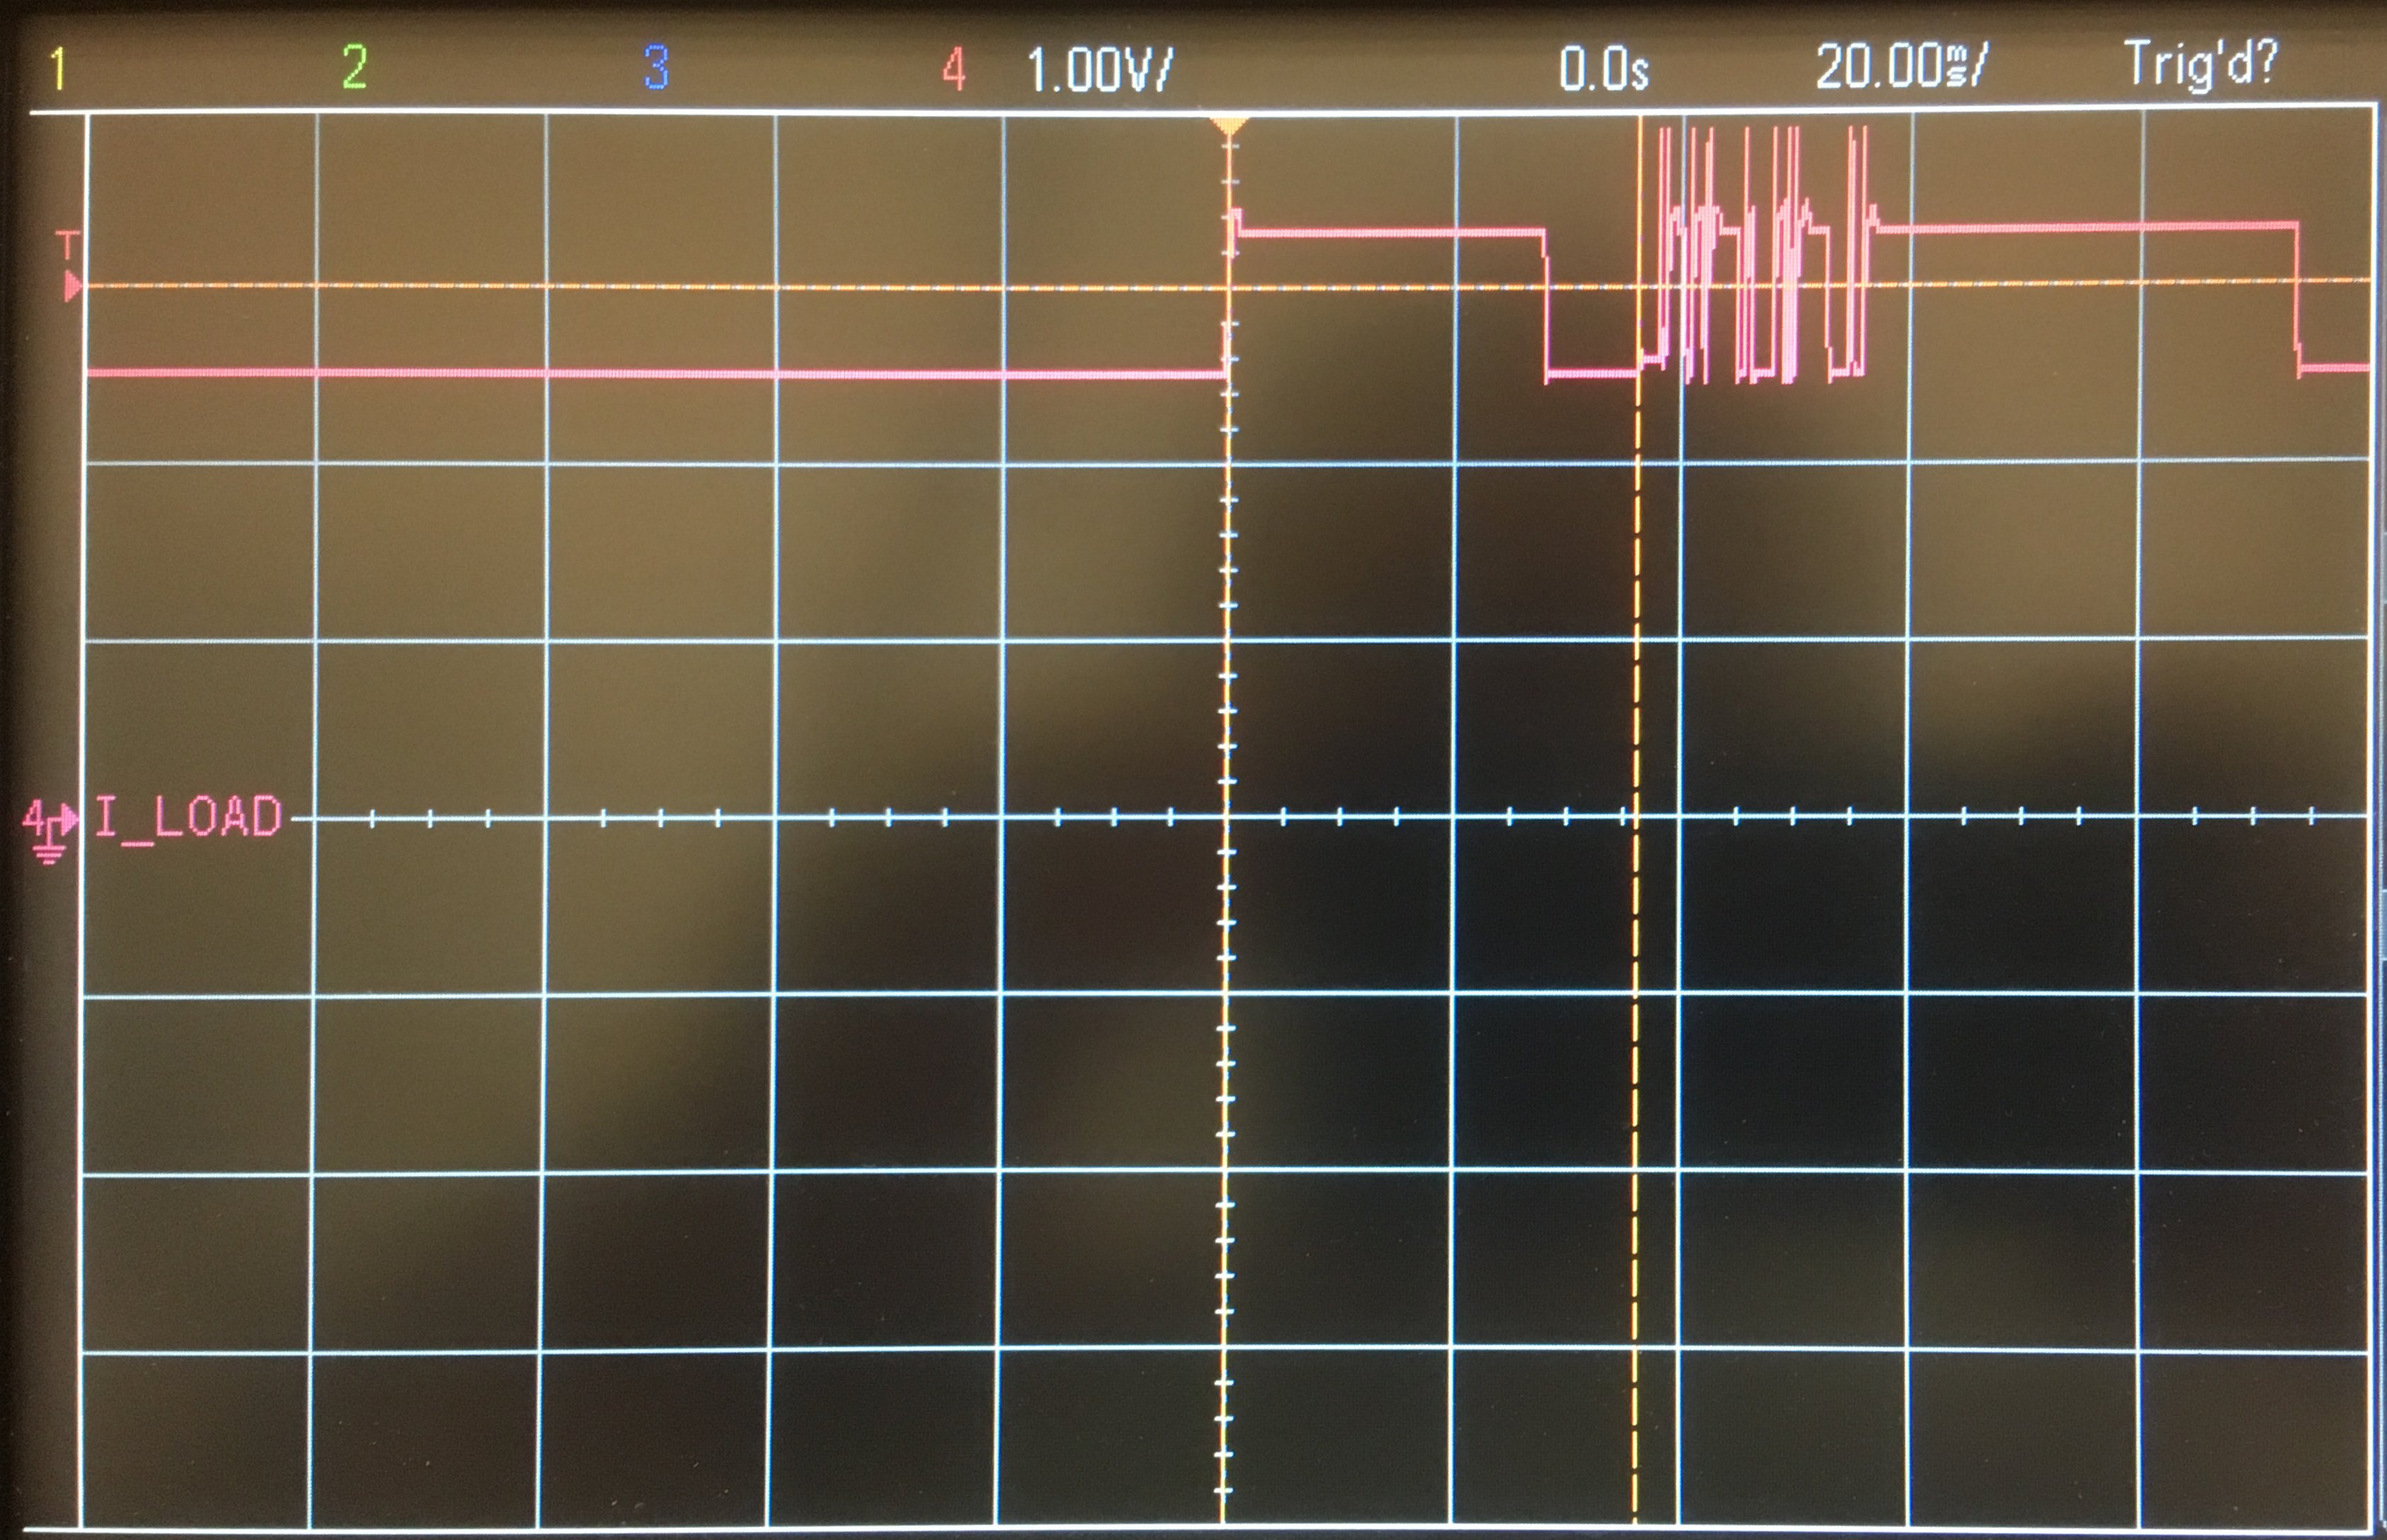
\includegraphics[width=\linewidth]
                {./res/current_transient/loss_of_lock-zoom2.jpg}
        };
        \draw (zoom2.south west) rectangle (zoom2.north east);
    \end{tikzpicture}
    \caption{}
    \end{subfigure}
    %
    \caption[Loss of lock transient current, unrecoverable]{
        Loss of lock transient current.
        This DCB could not regain lock after the connection was restored.
        Measured on 007.
    }
\end{figure}

\begin{figure}[ht]
    \centering
    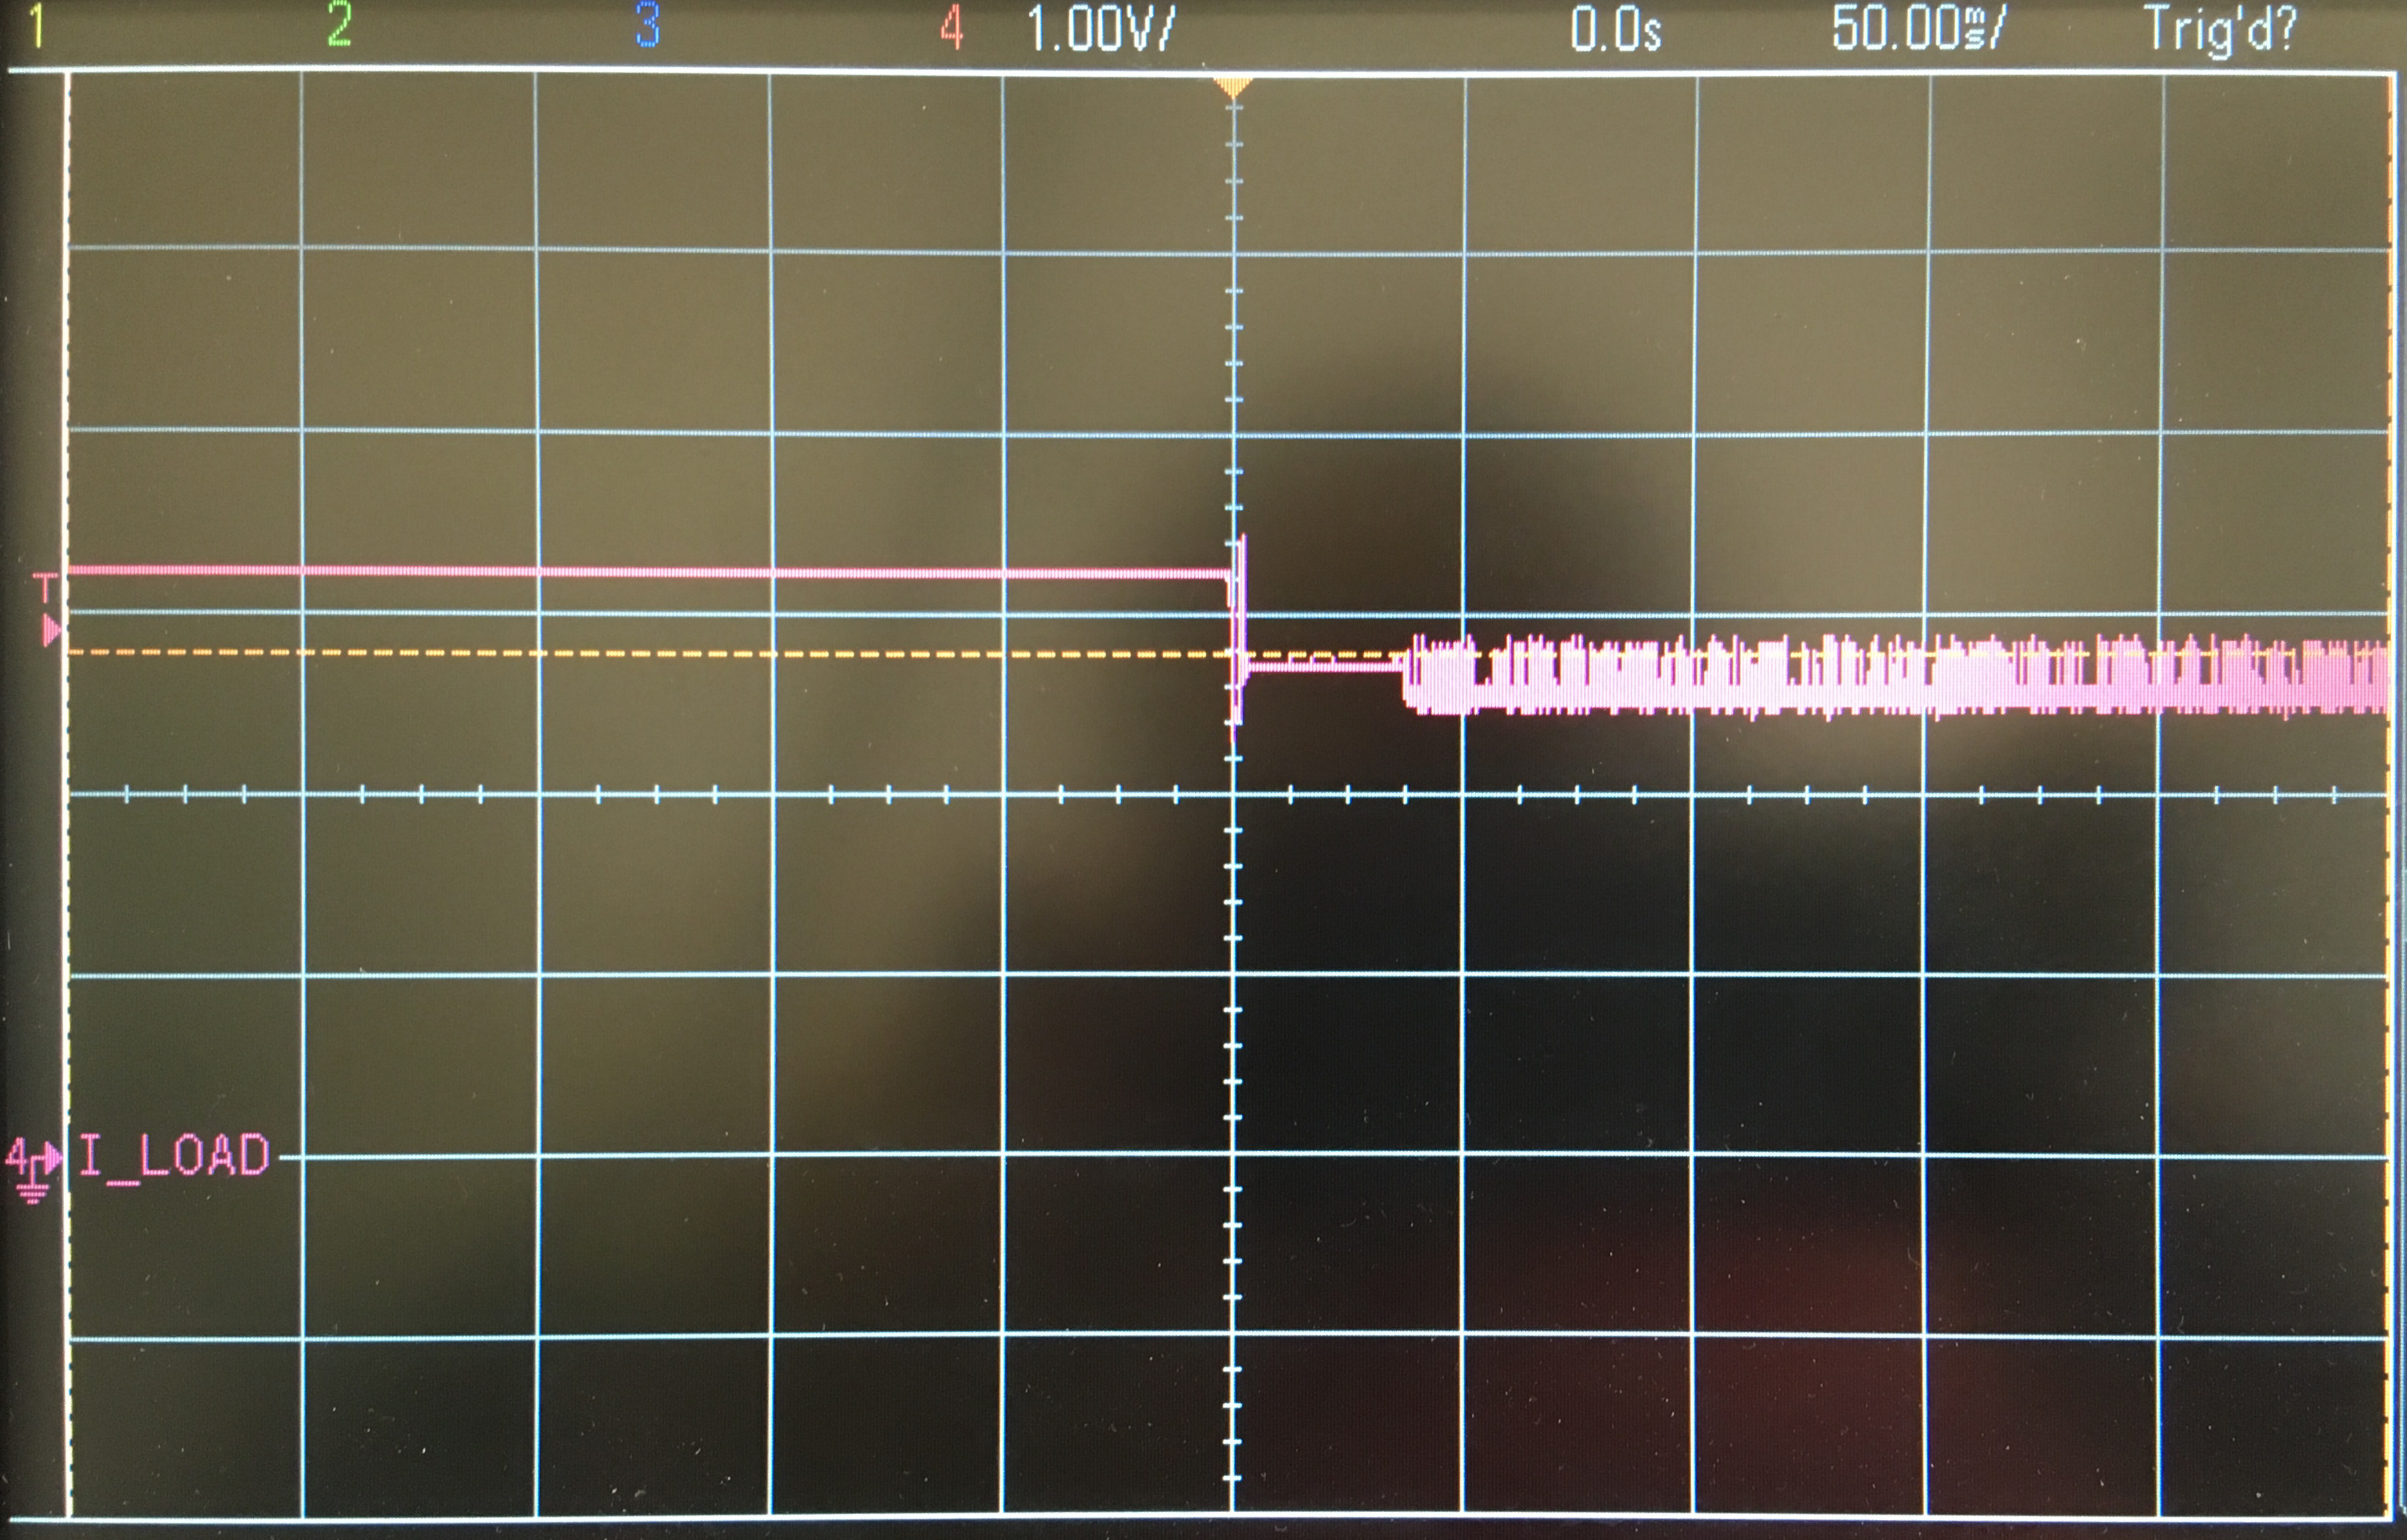
\includegraphics[width=0.8\linewidth]
        {./res/current_transient/loss_of_lock-recoverable.jpg}
    \caption[Loss of lock transient current, recoverable]{
        Loss of lock transient current.
        Only the data GBTx 5 and 6 were programmed.
        This DCB regained lock after the connection was restored.
        Measured on 008.
    }
\end{figure}

\begin{figure}[ht]
    \centering
    \begin{subfigure}{0.8\linewidth}
    \begin{tikzpicture}[boximg]
        \node [anchor=south west] (main) {
            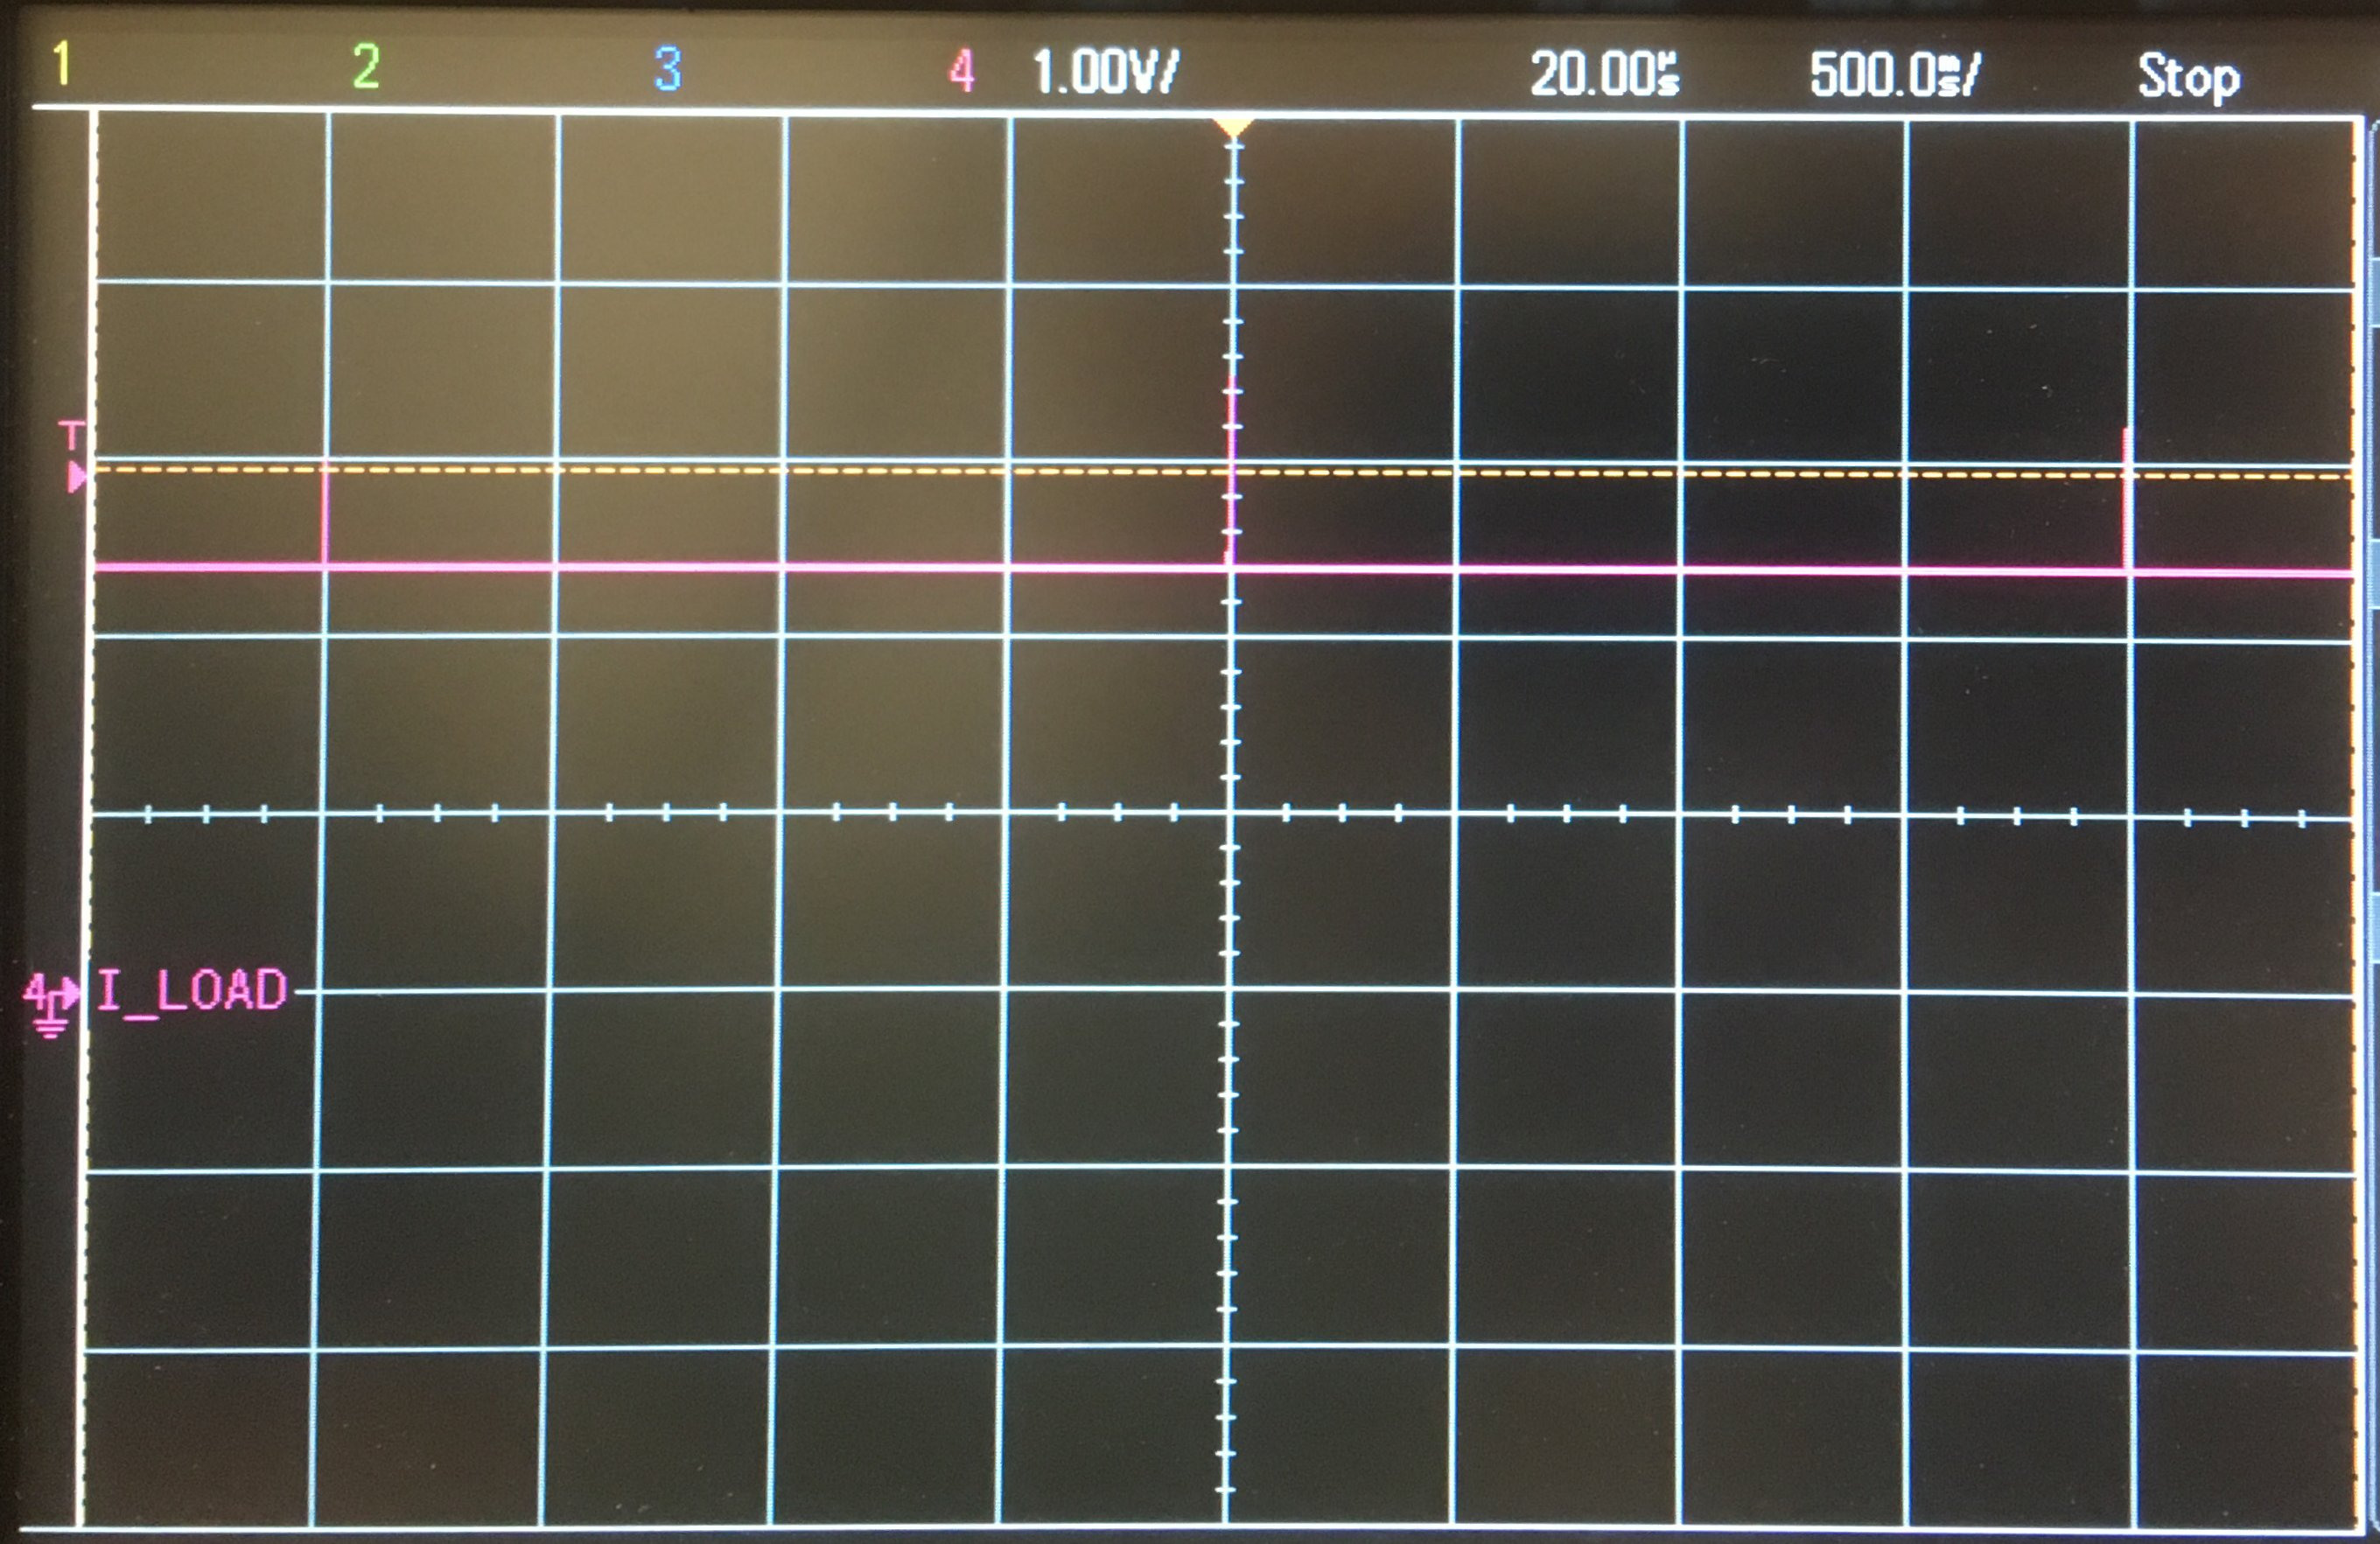
\includegraphics[width=\linewidth]
            {./res/current_transient/during_loss_of_lock.jpg}
        };
        \begin{scope}[x=(main.south east),y=(main.north west)]
            \node [draw,red,minimum height=4.5em, minimum width=1.5em]
                (zoombox1) at (0.52,0.7) {};
        \end{scope}
    \end{tikzpicture}
    \caption{}
    \end{subfigure}
    %
    \\[0.5\baselineskip]
    %
    \begin{subfigure}{0.42\linewidth}
    \begin{tikzpicture}[boximg,red]
        \node [anchor=south west] (zoom1) {
            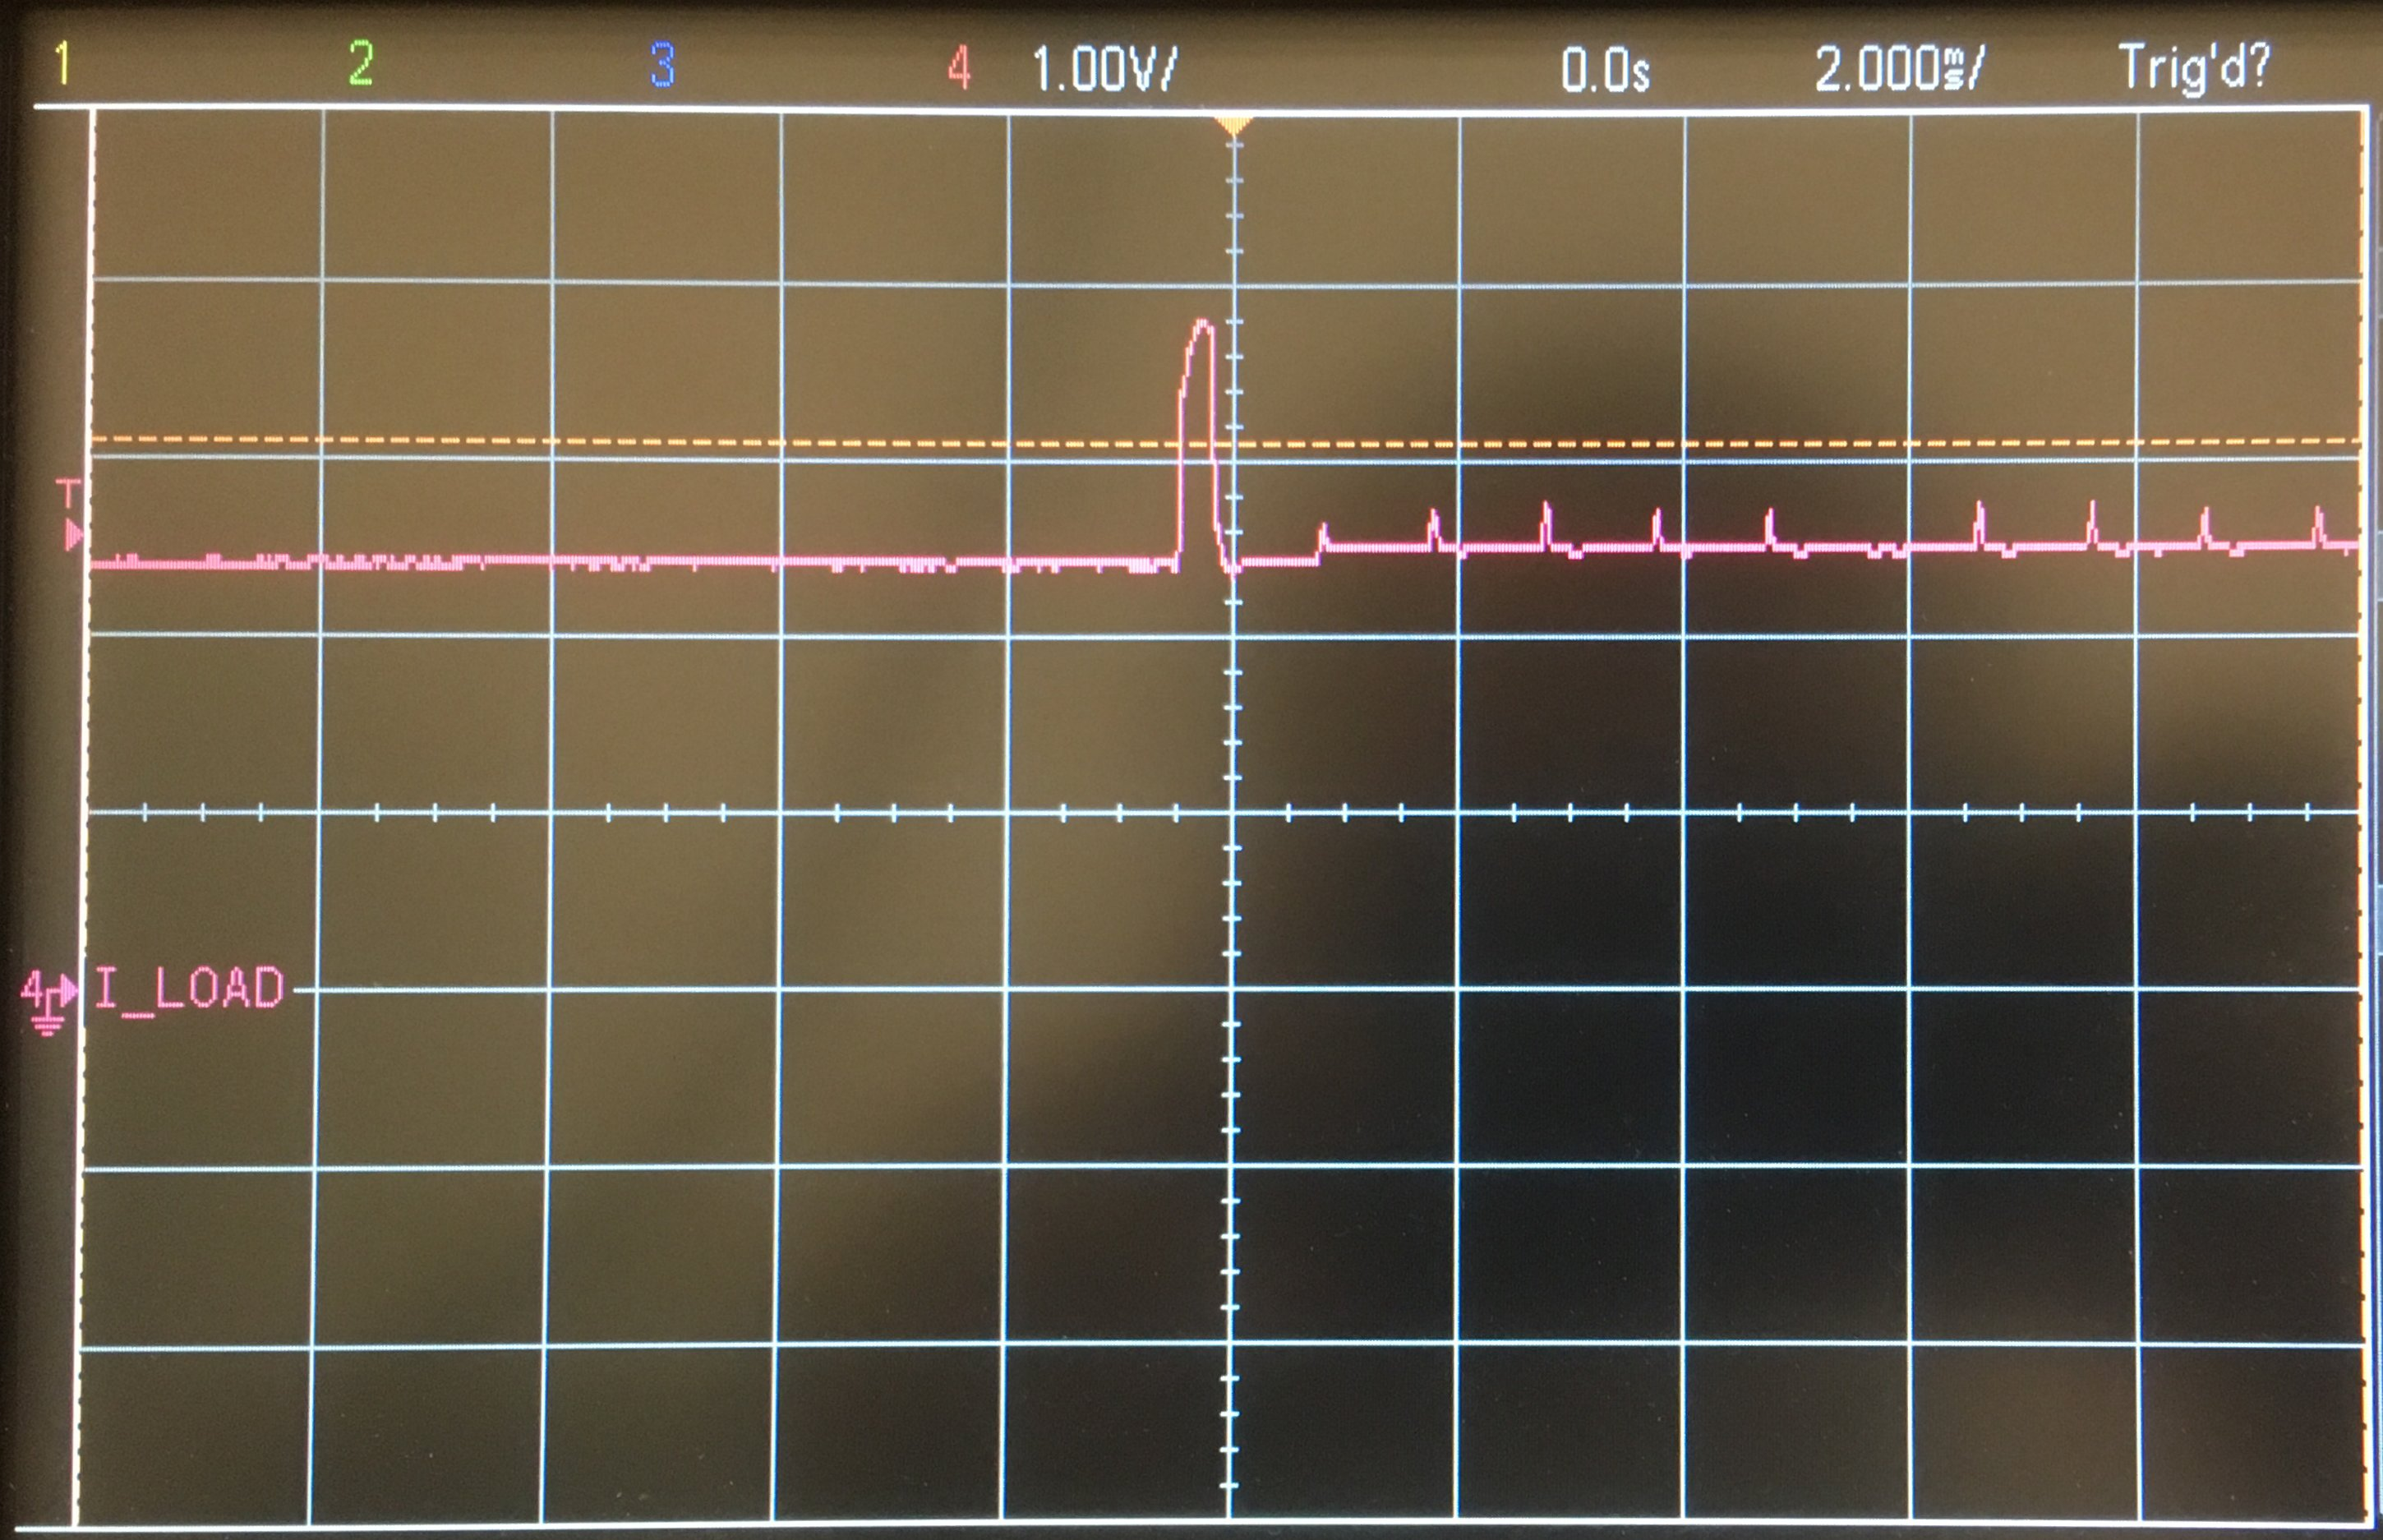
\includegraphics[width=\linewidth]
                {./res/current_transient/during_loss_of_lock-zoom.jpg}
        };
        \draw (zoom1.south west) rectangle (zoom1.north east);
        \begin{scope}[x=(zoom1.south east),y=(zoom1.north west)]
            \node [draw,green,minimum height=2em, minimum width=1em]
                (zoombox2) at (0.5,0.7) {};
        \end{scope}
    \end{tikzpicture}
    \caption{}
    \end{subfigure}
    %
    \hspace{0.04\linewidth}
    %
    \begin{subfigure}{0.32\linewidth}
    \begin{tikzpicture}[boximg,green]
        \node  (zoom2) {
            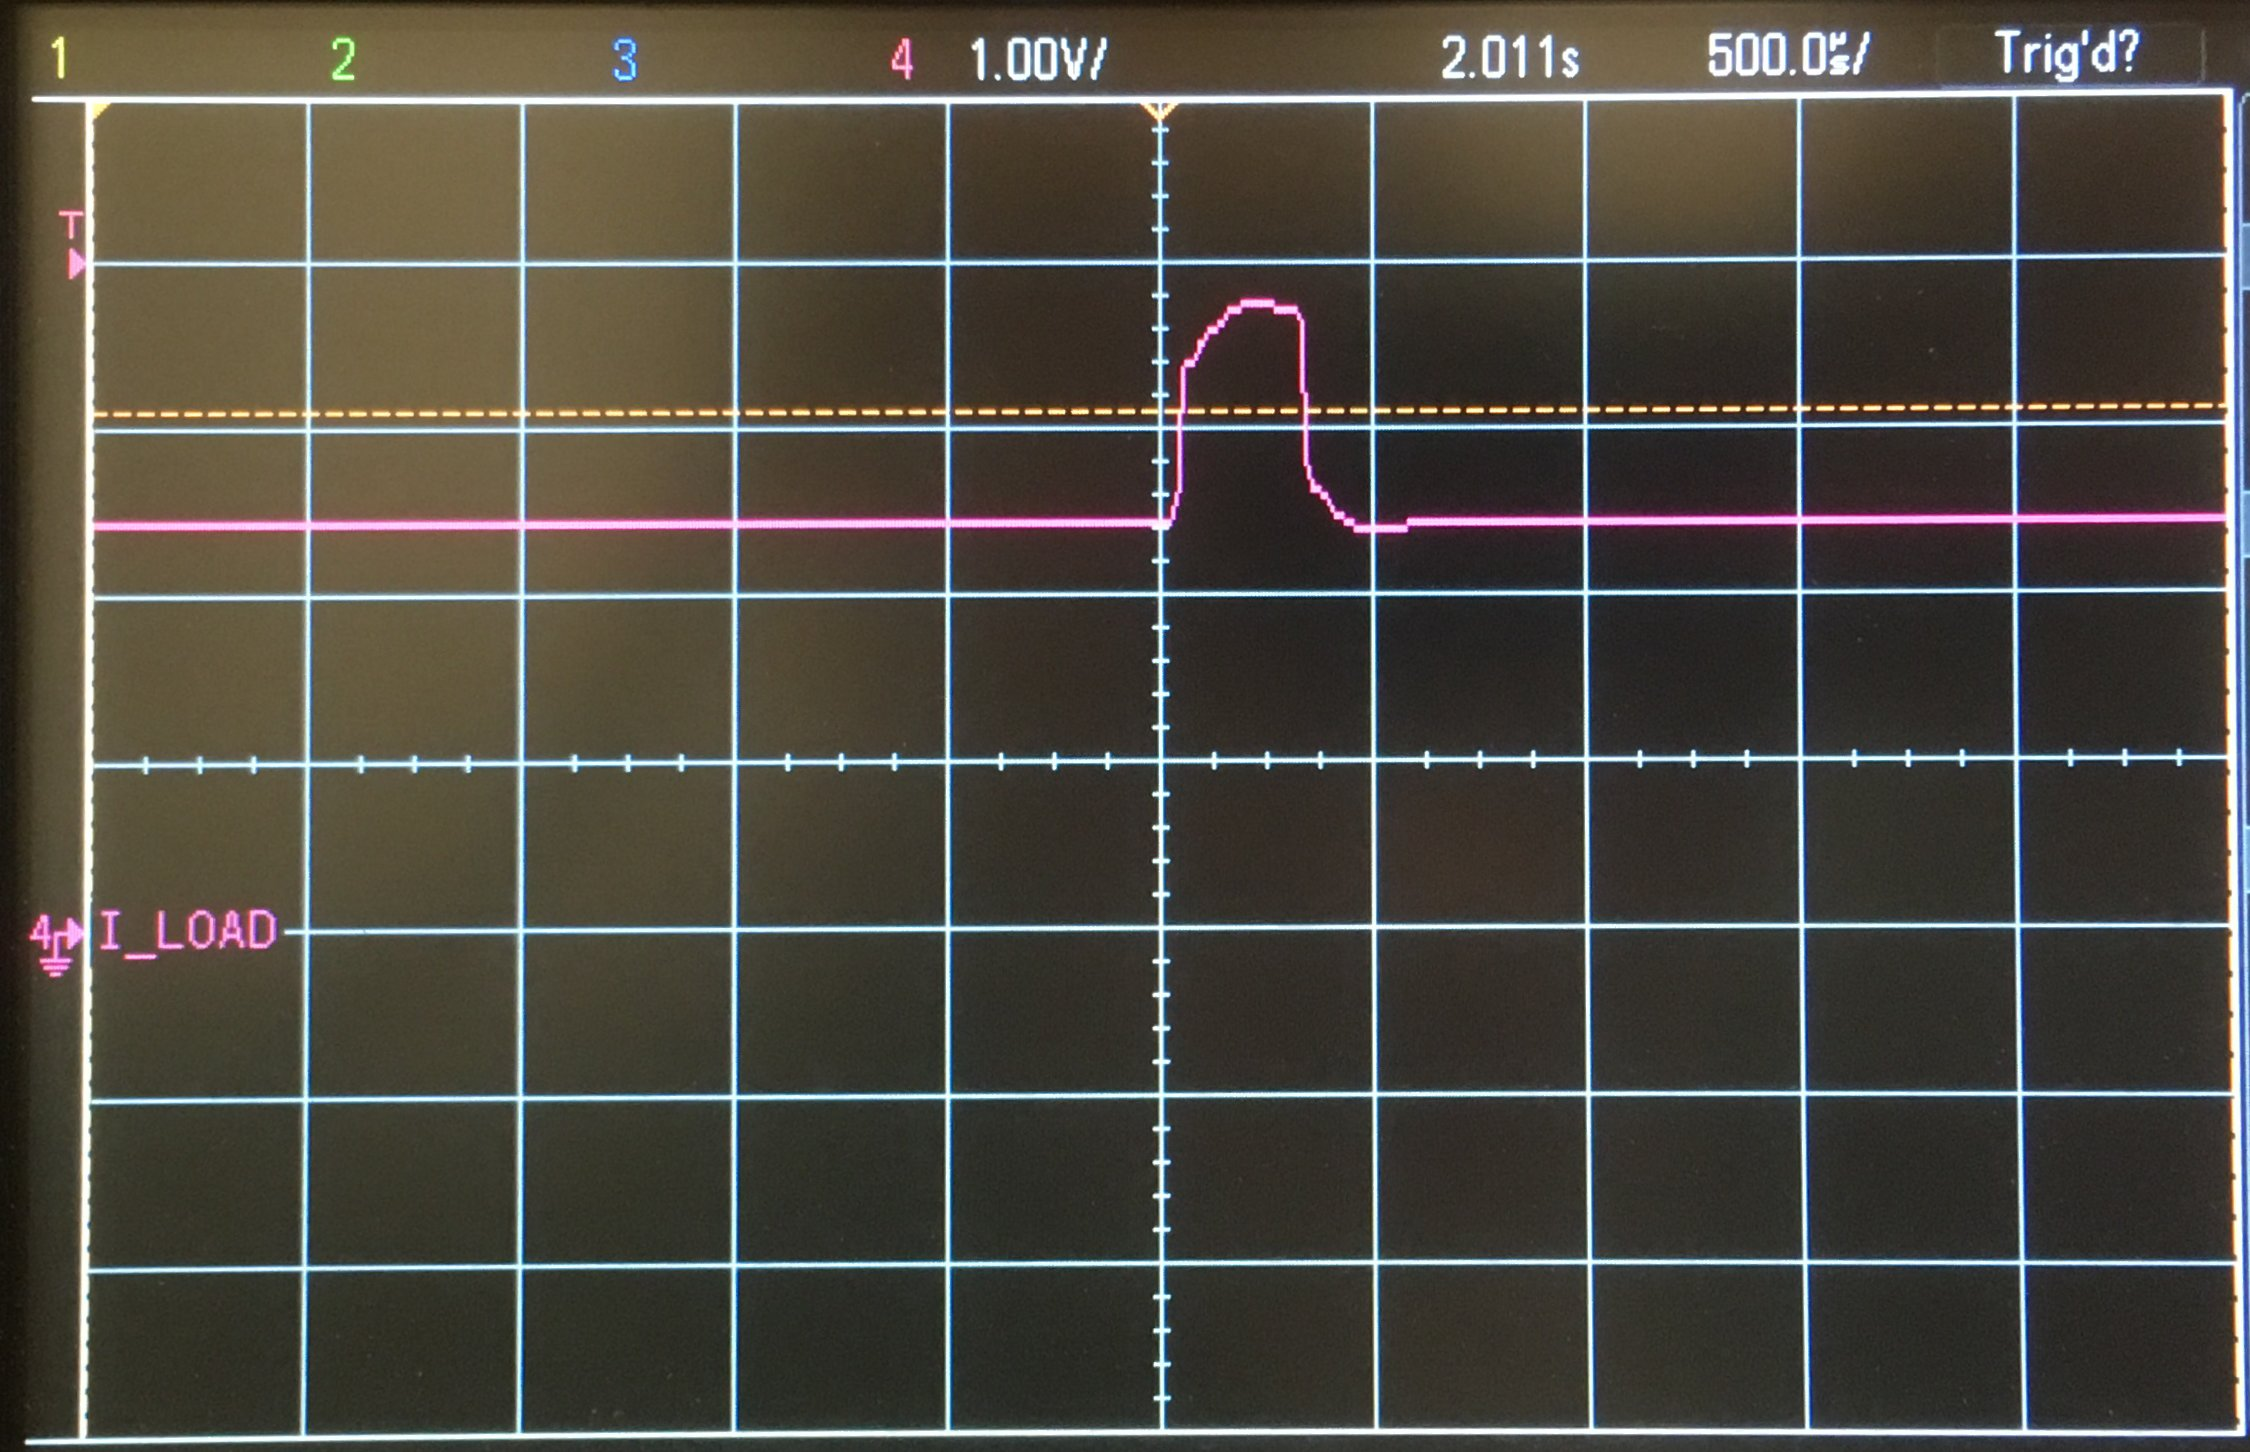
\includegraphics[width=\linewidth]
                {./res/current_transient/during_loss_of_lock-zoom-zoom.jpg}
        };
        \draw (zoom2.south west) rectangle (zoom2.north east);
    \end{tikzpicture}
    \caption{}\label{DLOL-zz}
    \end{subfigure}
    %
    \caption[During loss of lock transient current, unrecoverable]{
        During loss of lock transient current.
        DCB 007 in this stage is cleaner than DCB 008, but it could not recover
        after the connection is reestablished.
        Measured on 007.
    }
\end{figure}

\begin{figure}[ht]
    \centering
    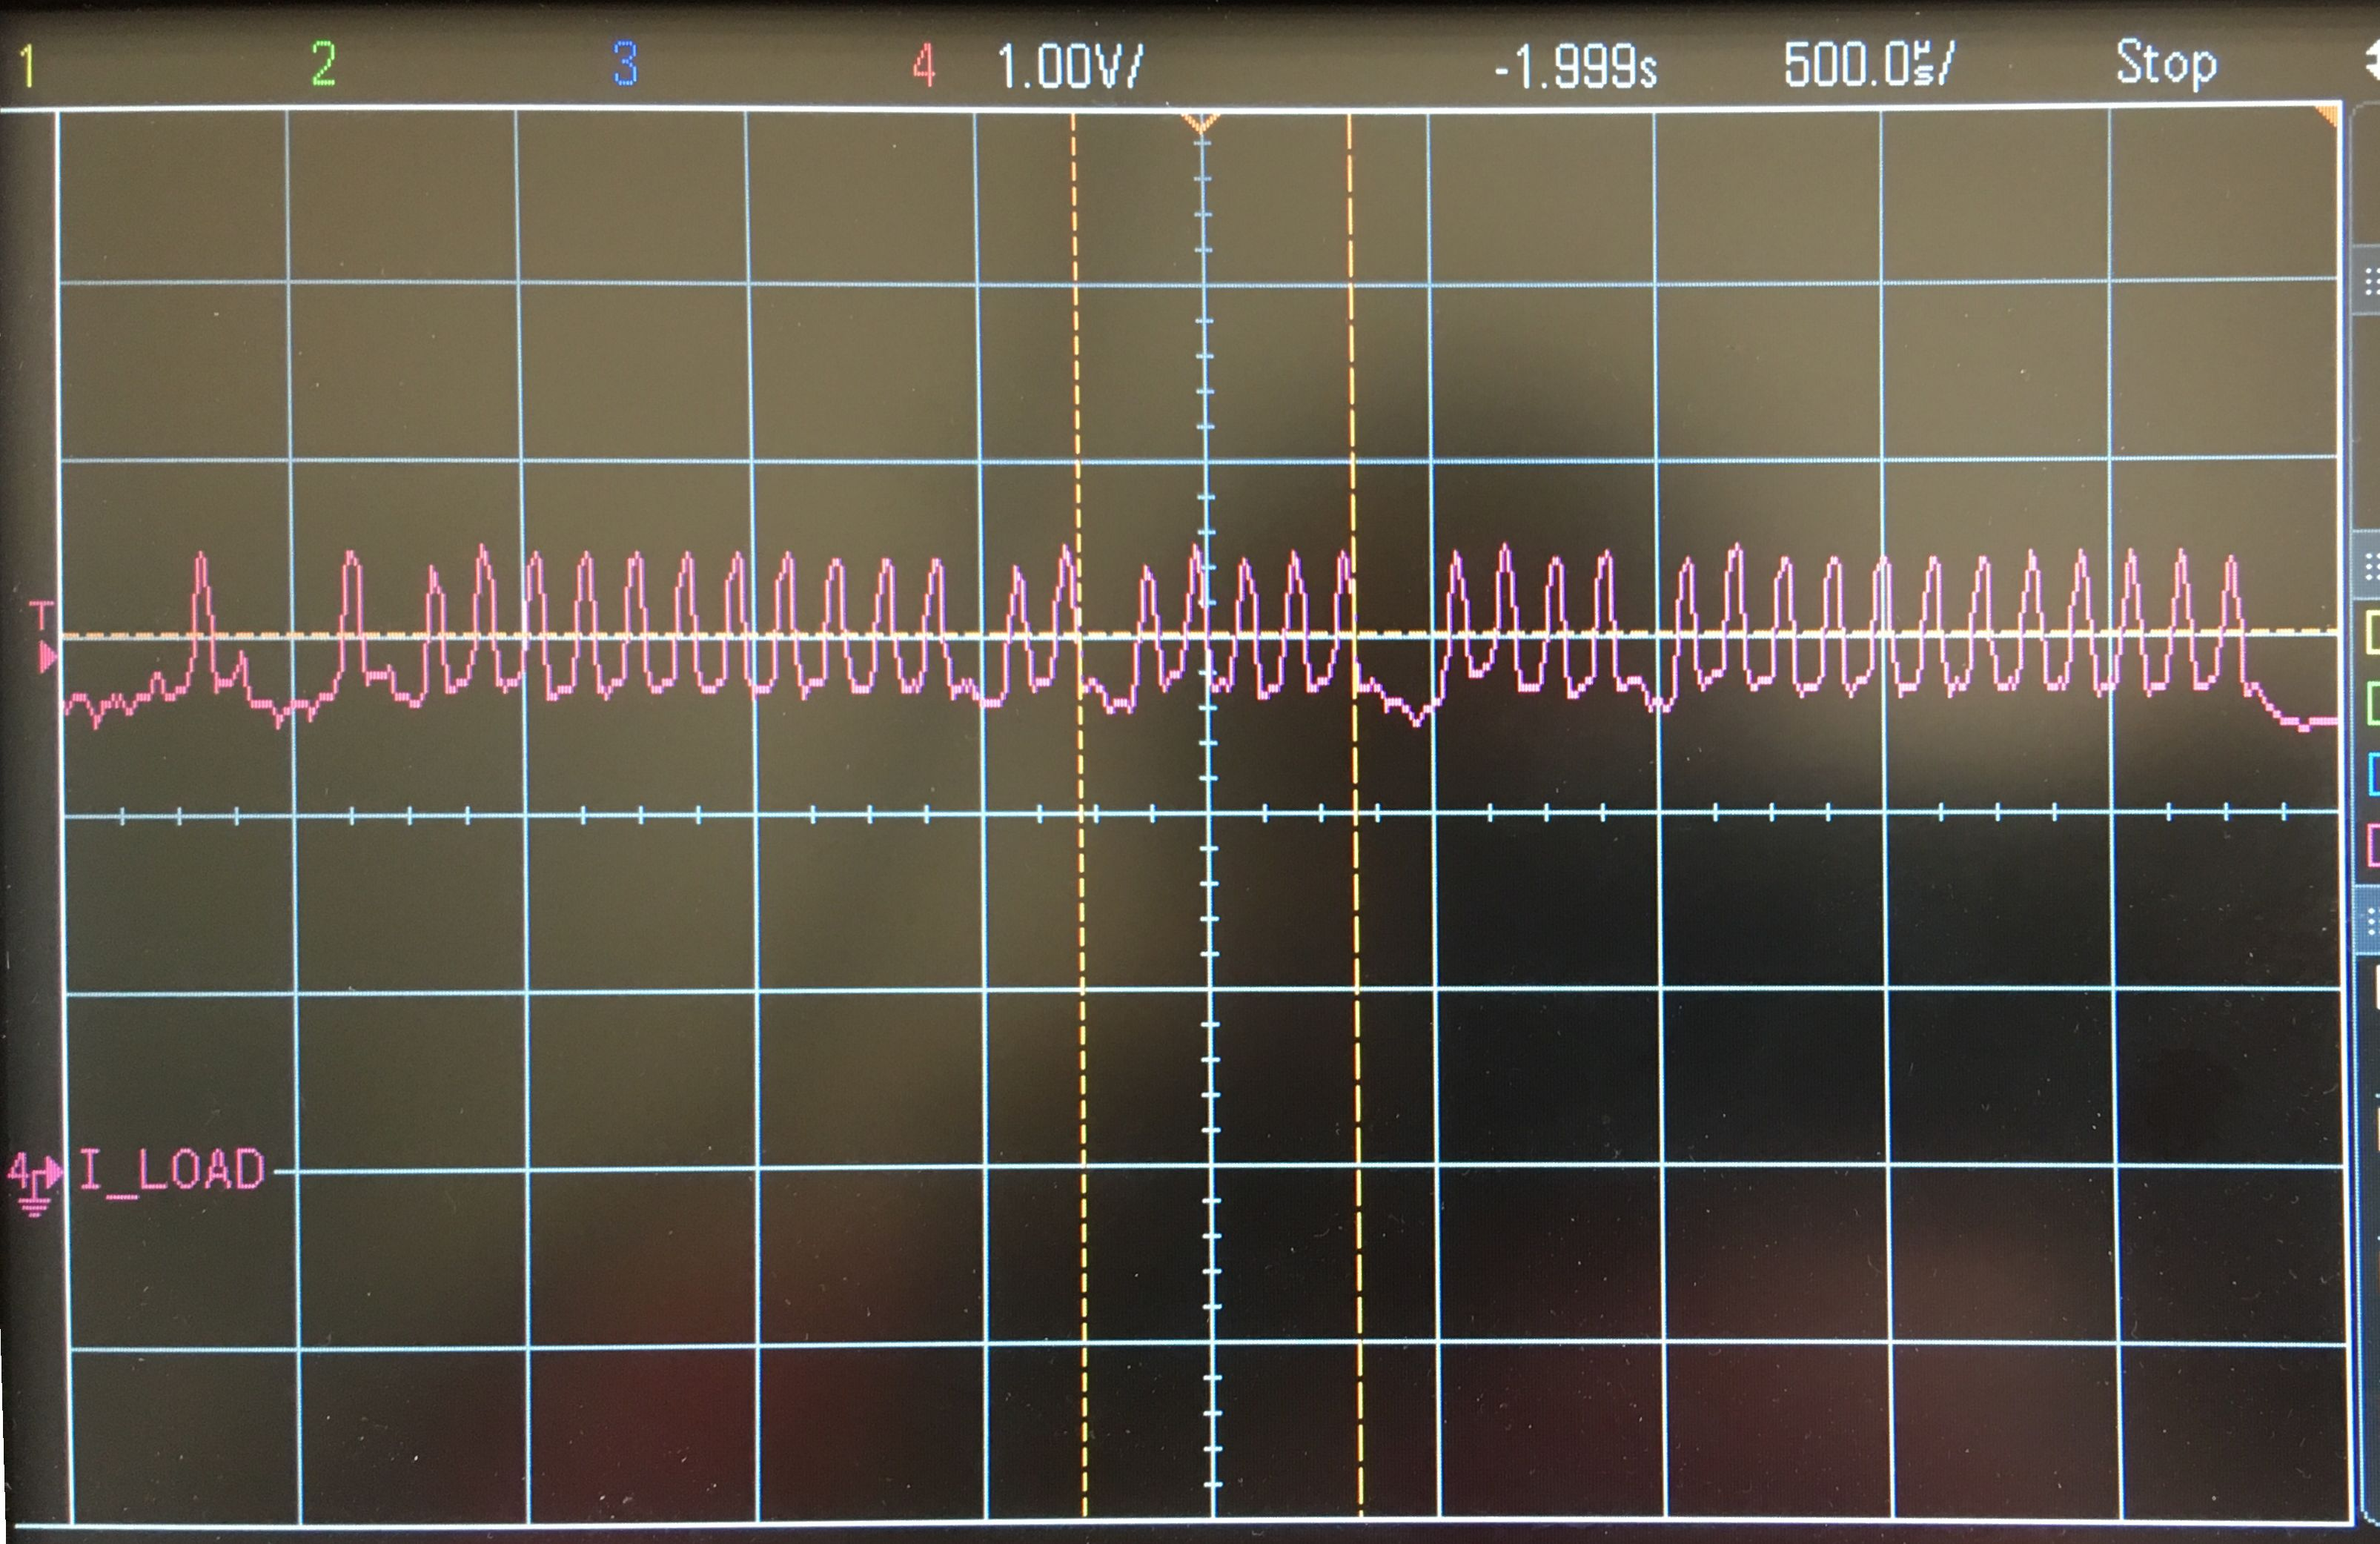
\includegraphics[width=0.8\linewidth]
        {./res/current_transient/during_loss_of_lock-recoverable.jpg}
    \caption[During loss of lock transient current, recoverable]{
        During Loss of lock transient current.
        This DCB regained lock after the connection was restored.
        Measured on 008.
        Note that the timescale is the same as in \autoref{DLOL-zz}.
    }
\end{figure}

\begin{figure}[ht]
    \centering
    \begin{subfigure}{0.8\linewidth}
    \begin{tikzpicture}[boximg]
        \node [anchor=south west] (main) {
            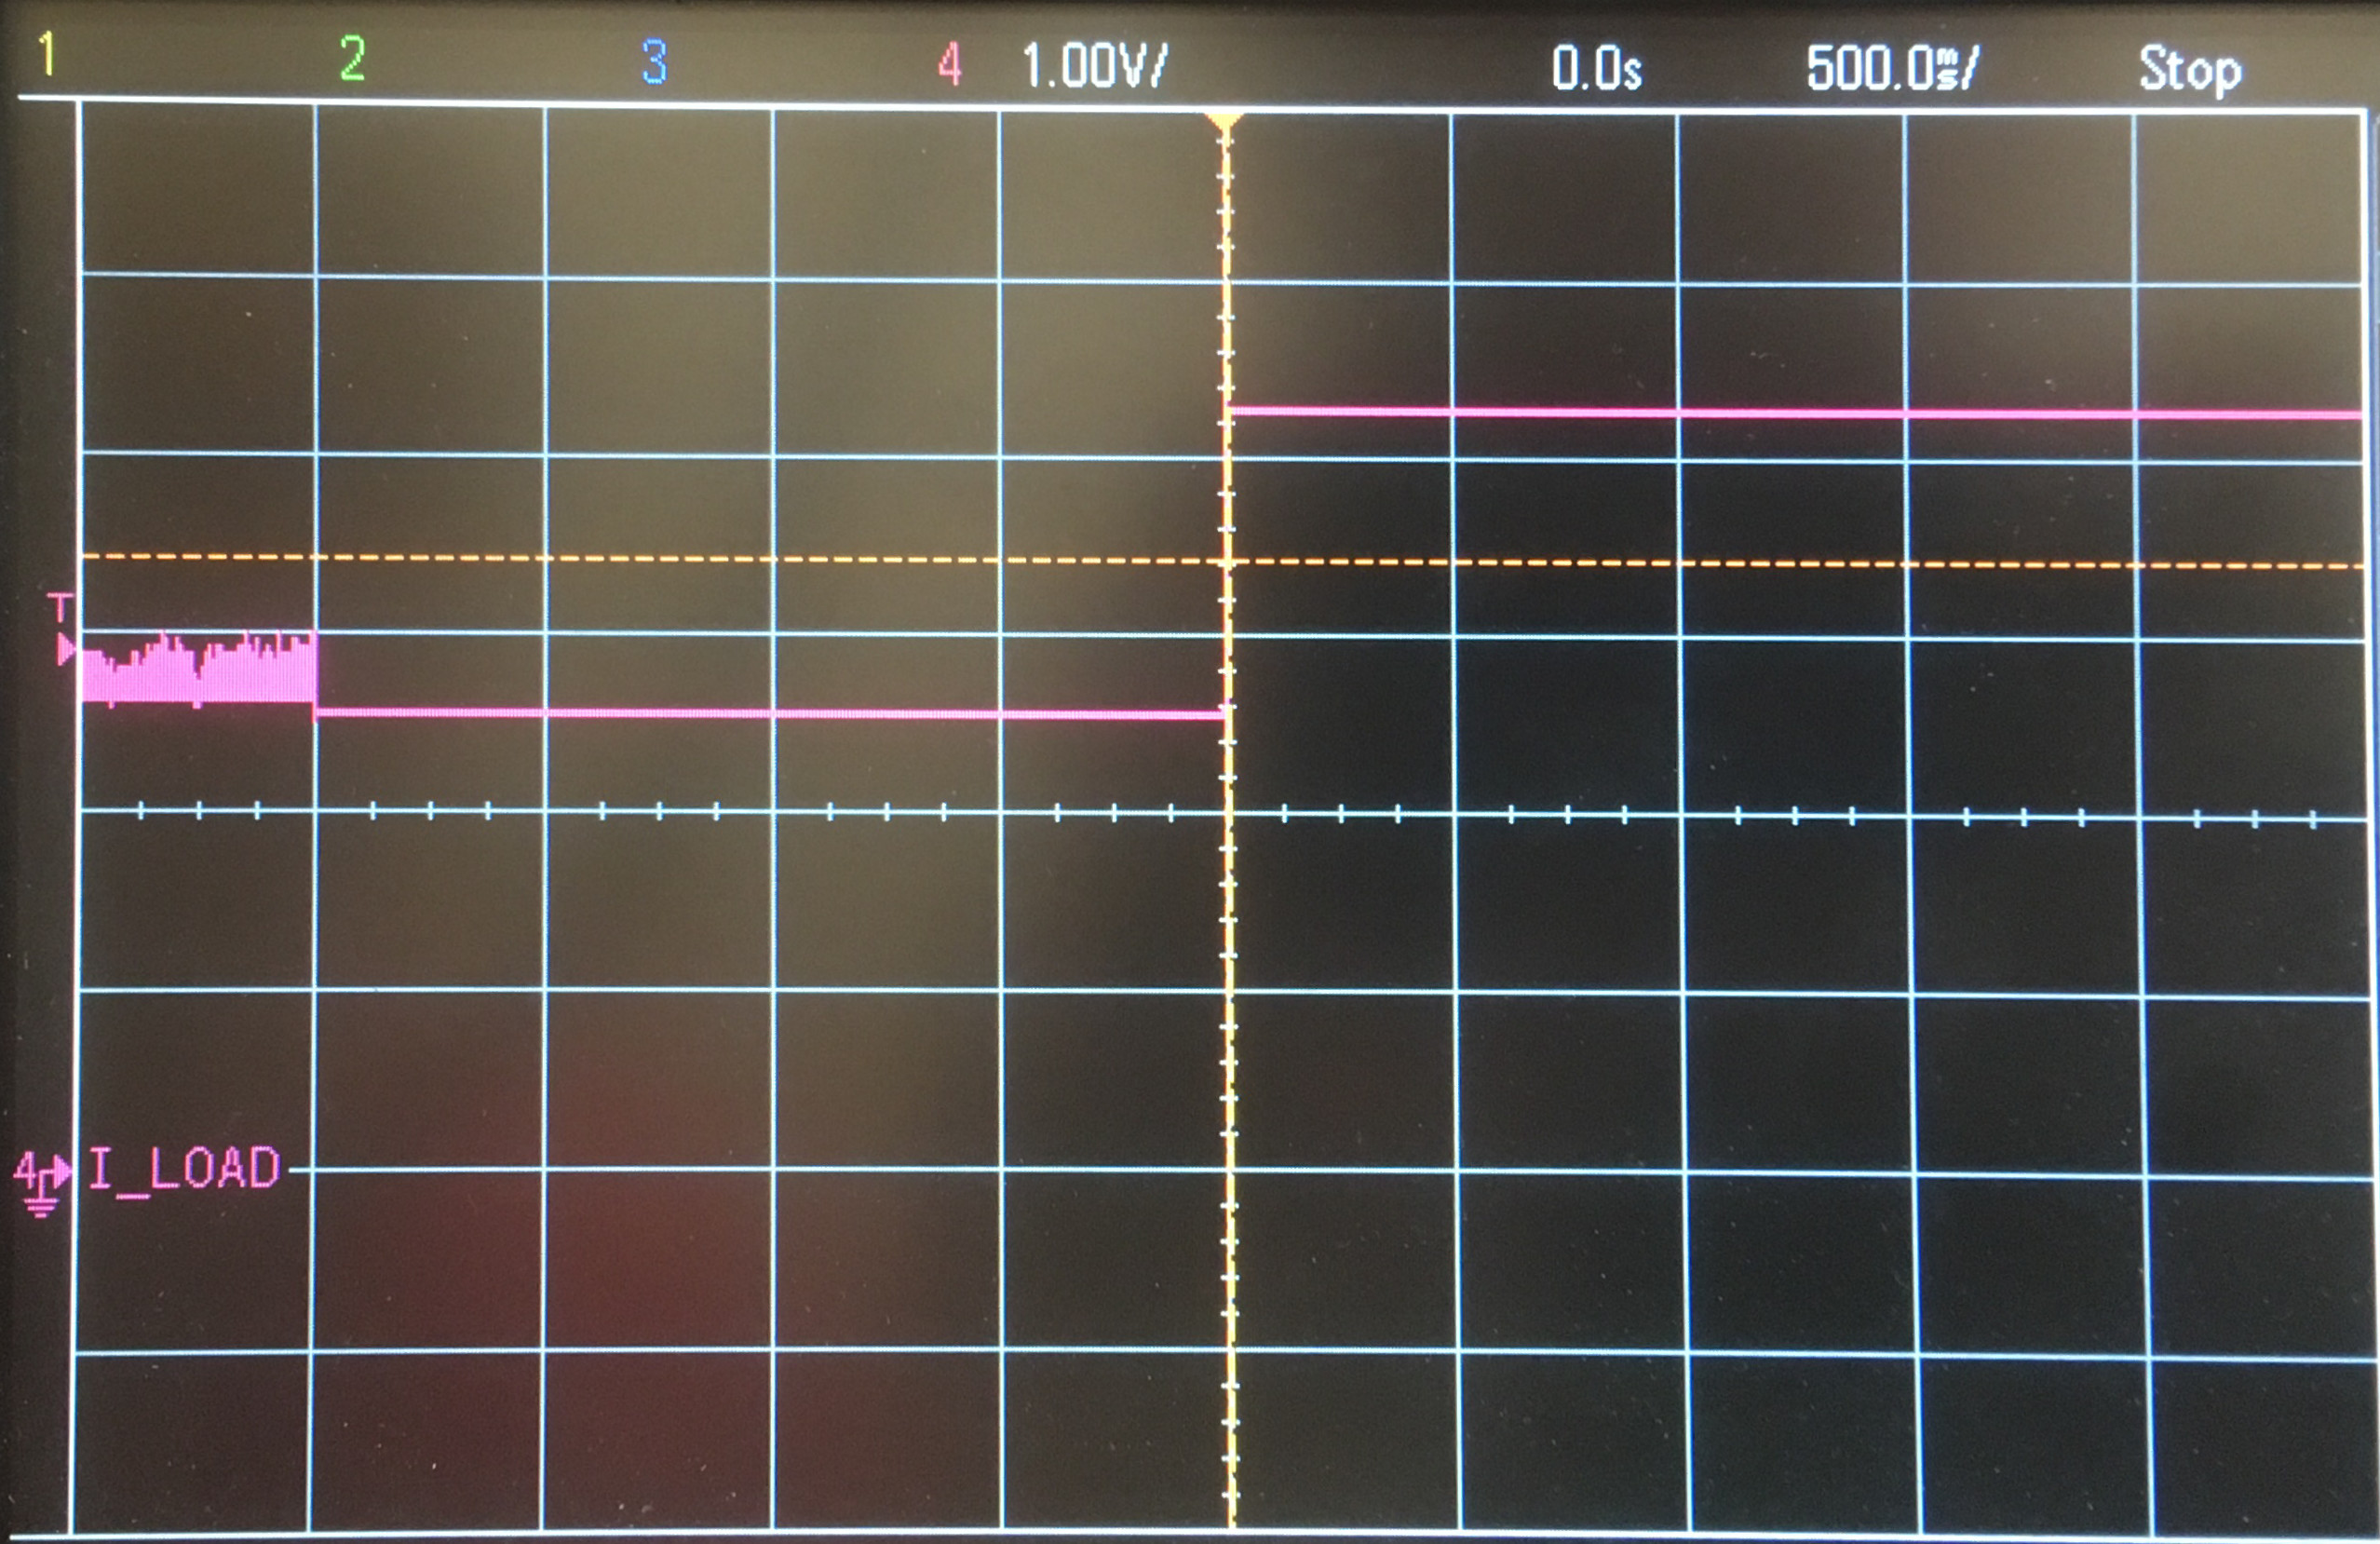
\includegraphics[width=\linewidth]
                {./res/current_transient/regain_of_lock.jpg}
        };
        \begin{scope}[x=(main.south east),y=(main.north west)]
            \node [draw,red,minimum height=5em, minimum width=2em] (zoombox1)
                at (0.51,0.65) {};
        \end{scope}
    \end{tikzpicture}
    \caption{}
    \end{subfigure}
    %
    \\[0.5\baselineskip]
    %
    \begin{subfigure}{0.5\linewidth}
    \begin{tikzpicture}[boximg,red]
        \node (zoom1) {
            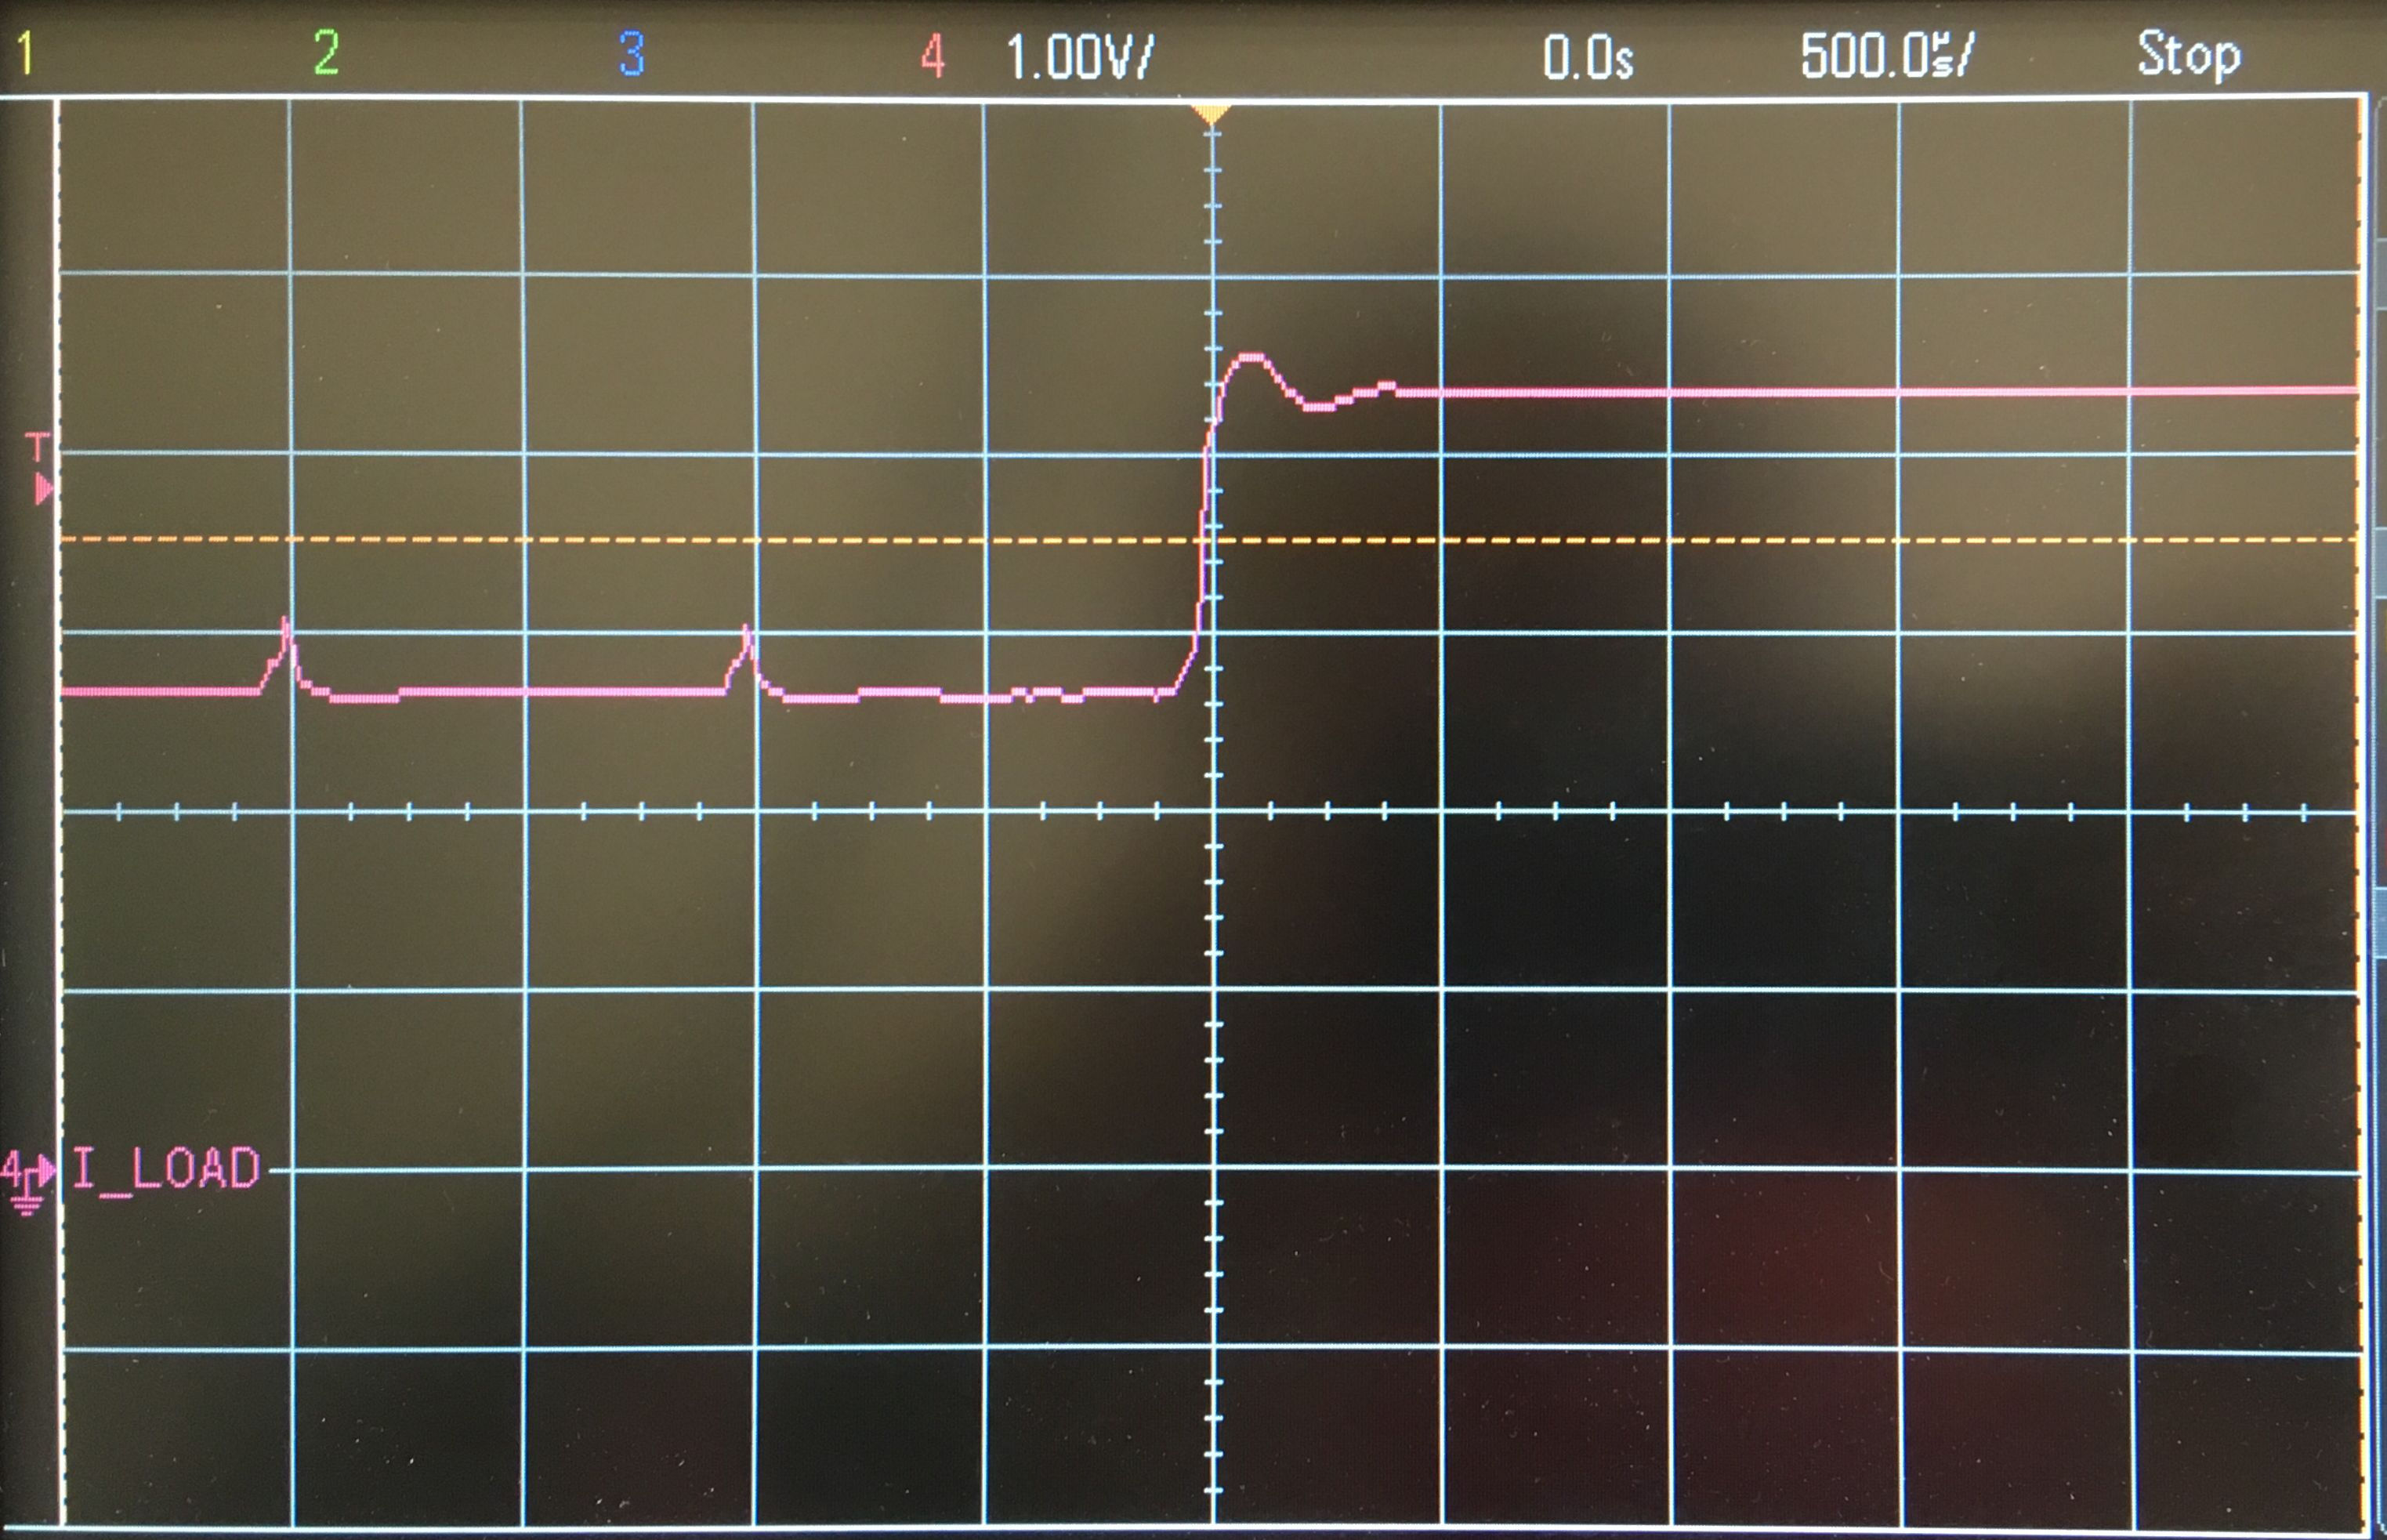
\includegraphics[width=\linewidth]
                {./res/current_transient/regain_of_lock-zoom.jpg}
        };
        \draw (zoom1.south west) rectangle (zoom1.north east);
    \end{tikzpicture}
    \caption{}
    \end{subfigure}
    \caption[Regain of lock transient current]{
        Currently 007 cannot regain lock, but 008 can.
        Note that during the loss of lock stage, 008 is much more noisy.
        Measured on 008.
    }
\end{figure}


\section{Transient voltage}
\subsection{Transient voltage on \SI{1.5}{\volt}}
We used a differential probe to measure the \SI{1.5}{\volt} rail on the DCB
directly.
We found a particular pair of contact, and handheld the probe to do the
measurements.

\begin{figure}[ht]
    \centering
    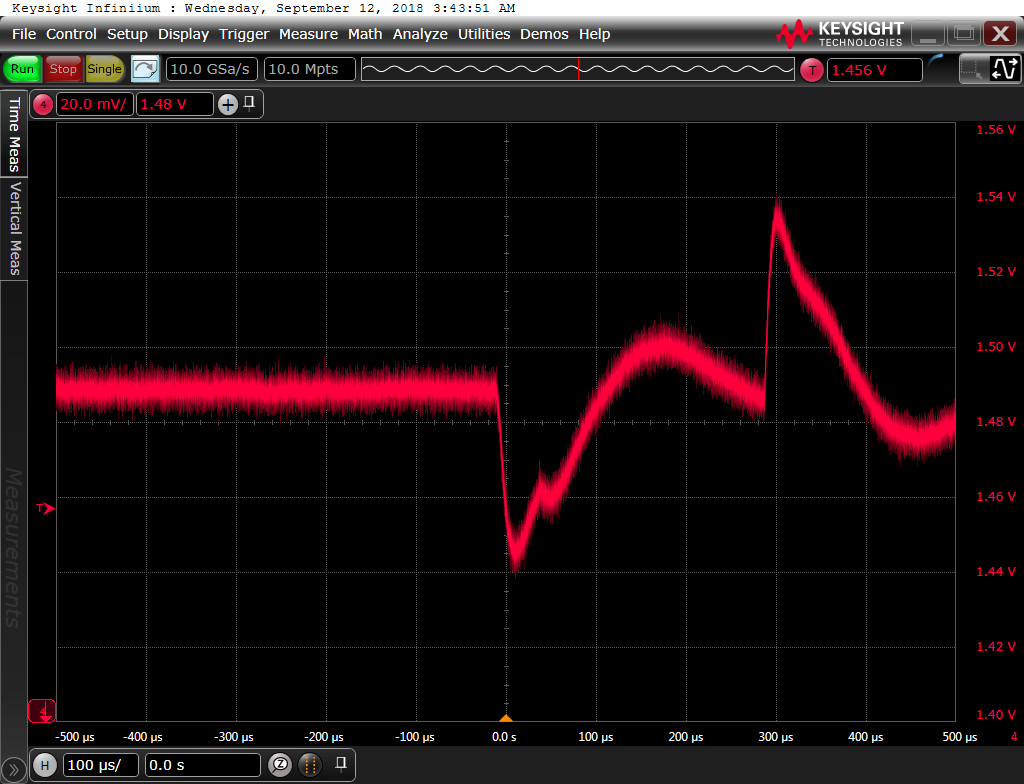
\includegraphics[width=0.8\linewidth]
        {./res/voltage_transient/time_out.png}
    \caption[Voltage transient due to timeout]{
        We have enabled timeout on master GBTx, and it would kick in every 2
        seconds.
        Timeout would reset\protect\footnotemark the GBTx.
        Measured on 007.
    }
\end{figure}

\footnotetext{Not sure if it means that the FSM would go back to state 0. This
statement comes from GBTx expert Daniel Hernandez.}

\subsection{Transient voltage on data GBTxs}
The \texttt{TX\_RDY} signals for all data GBTxs were brought out to the FFC
breakout boards.
We plugged in 2 differential probes on 2 of the breakout boards, and measured
that signal for data GBTxs 5 and 6.
During the measurement, only these 2 data GBTxs were programmed, due to the fact
that DCB 007 cannot regain lock if all 6 data GBTxs were all programmed.
DCB S/N pilot 007, 008 were used.

For DCB 007, \texttt{TX\_RDY} was still almost always asserted even if the
\SI{2.5}{\volt} rail was turned off, and was reasserted every 2 seconds.

For DCB 008, if the \SI{2.5}{\volt} was turned off, \texttt{TX\_RDY} was never
asserted, until the connection was restored; if only unplugging the master's
fibers, its behavior was the same as that of DCB 007.

\begin{figure}[ht]
    \centering
    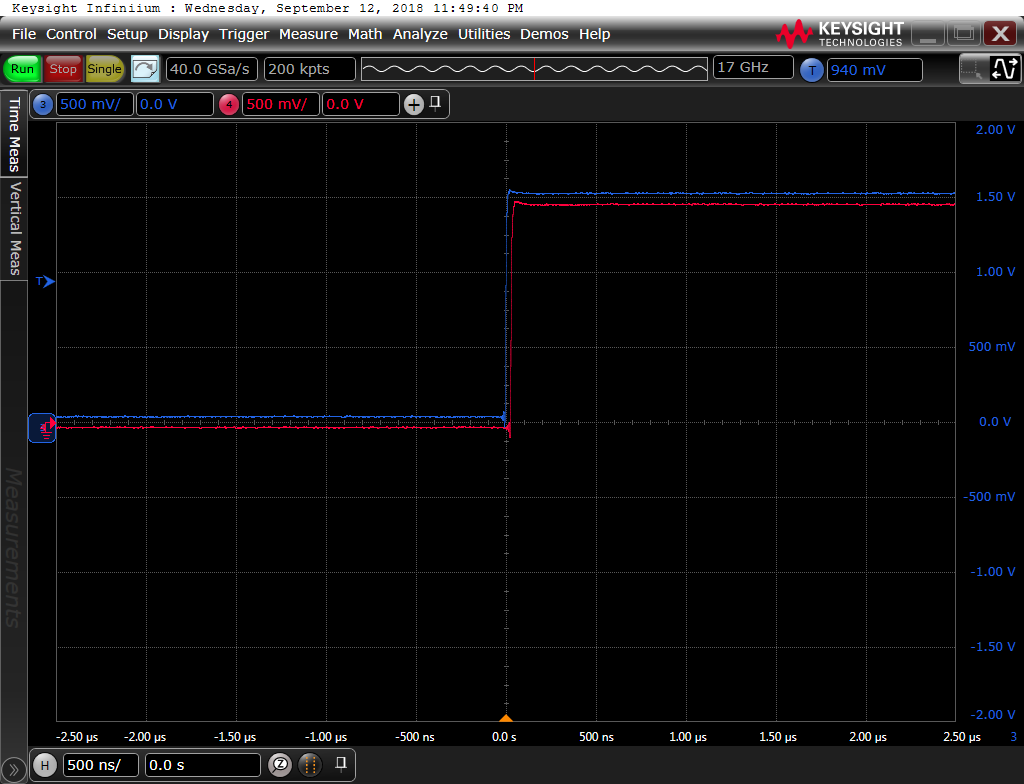
\includegraphics[width=0.8\linewidth]
        {./res/voltage_transient/txrdy.png}
    \caption[\texttt{TX\_RDY} signal on regain of lock, almost simutaneously]{
        This DCB was able to regain lock.
        Only the data GBTx 5 and 6 were programmed.
        Measured on 007.
    }
\end{figure}

\begin{figure}[ht]
    \centering
    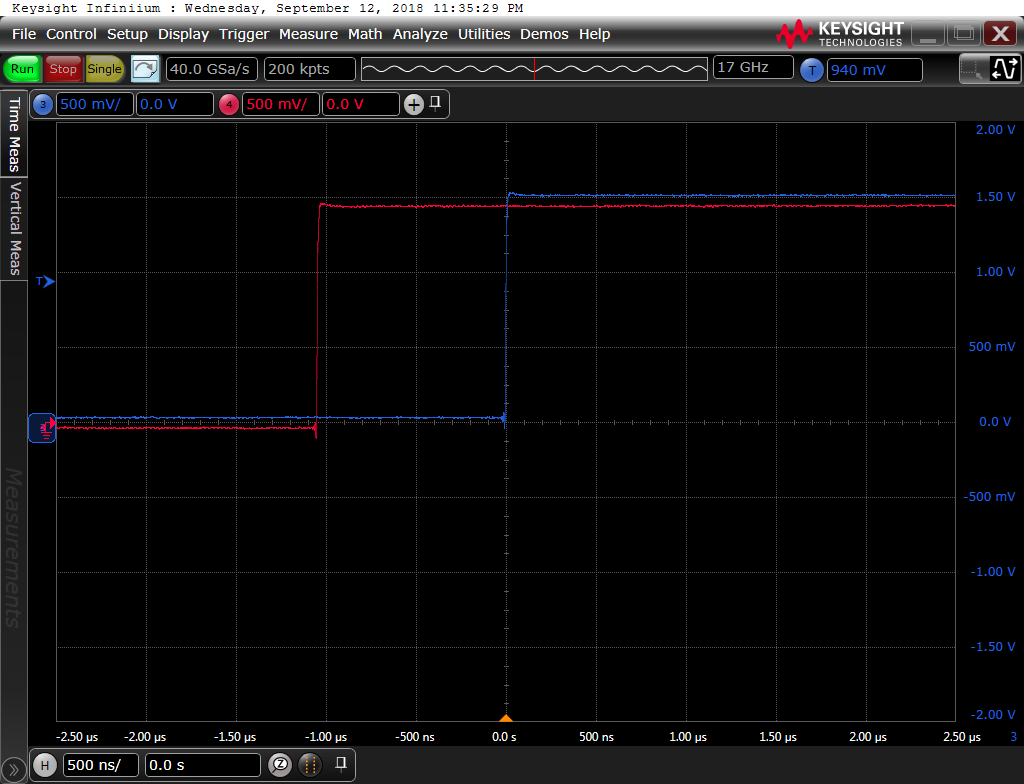
\includegraphics[width=0.8\linewidth]
        {./res/voltage_transient/txrdy_recoverable.png}
    \caption[\texttt{TX\_RDY} signal on regain of lock, larger temperal
            separation]{
        This DCB was able to regain lock.
        Only the data GBTx 5 and 6 were programmed.
        Measured on 008.
    }
\end{figure}


\section{Power-on reset voltage}
We used two probes, one probing the \SI{1.5}{\volt} rail voltage (Green), the
other probe the voltage of the \texttt{MC\_RESET\_B} pin.

\begin{figure}[ht]
    \centering
    \begin{subfigure}{0.8\linewidth}
    \begin{tikzpicture}[boximg]
        \node [anchor=south west] (main) {
            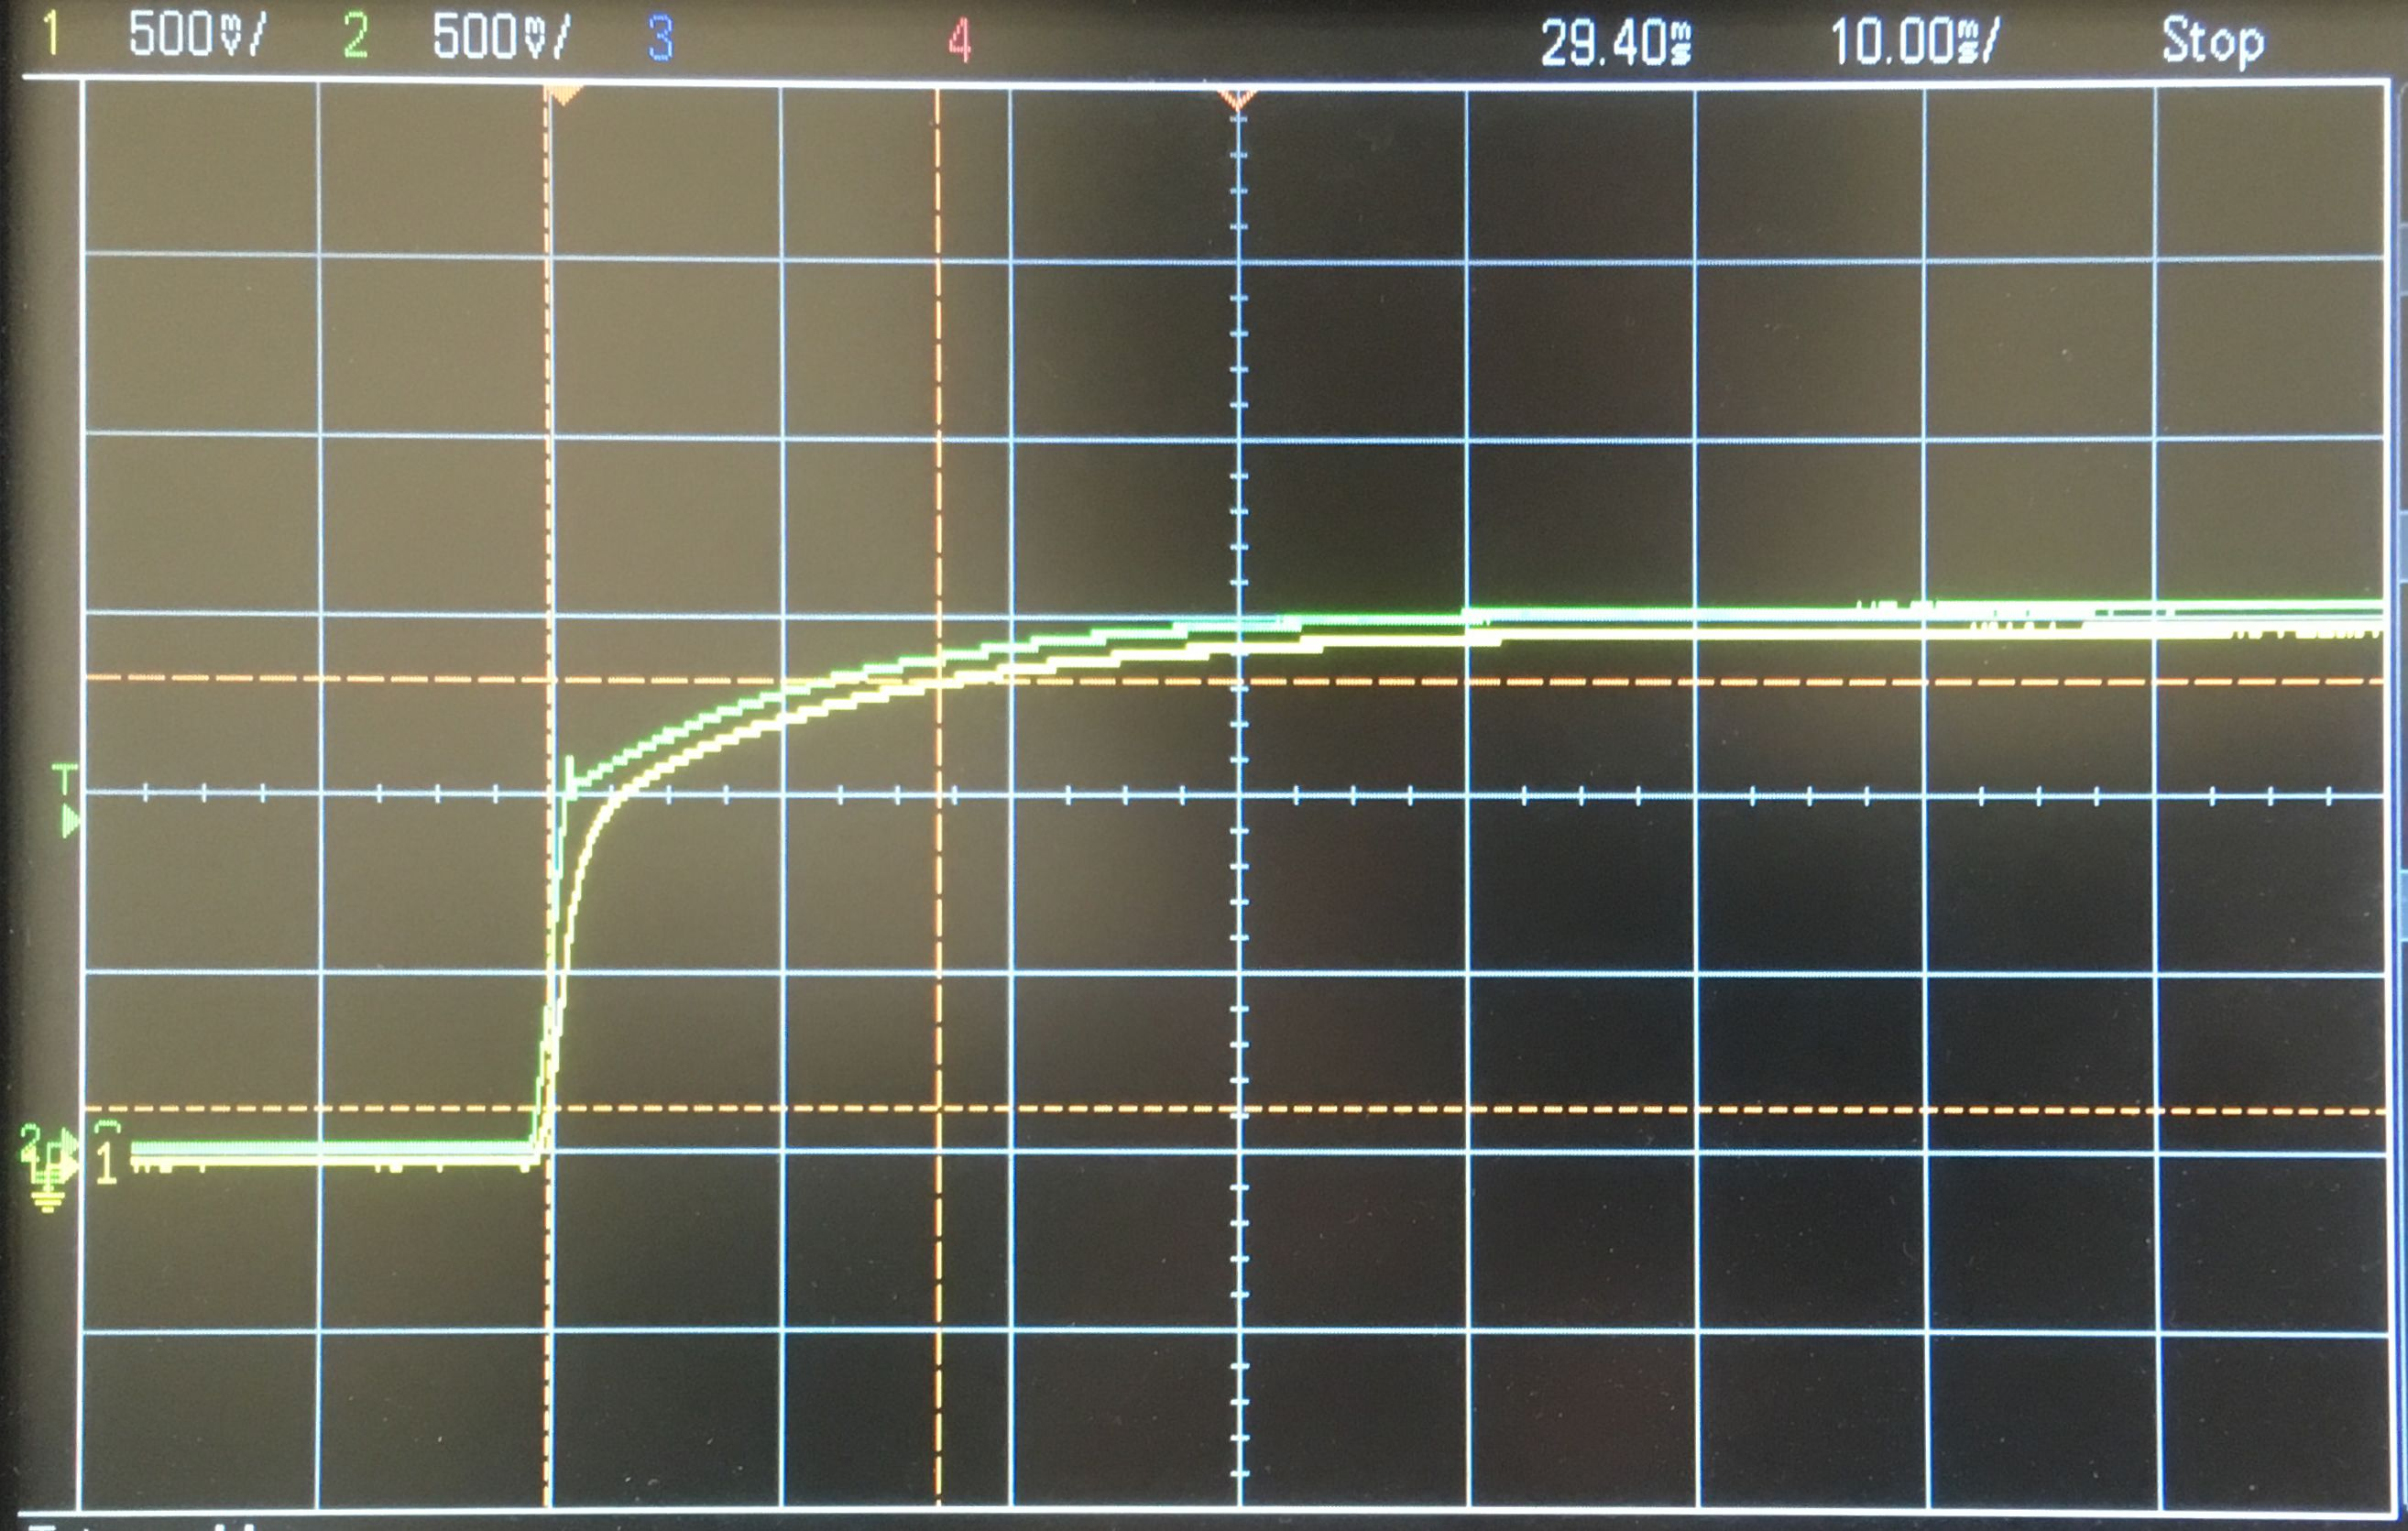
\includegraphics[width=\linewidth]
                {./res/power_on_reset/power_on_reset.jpg}
        };
        \begin{scope}[x=(main.south east),y=(main.north west)]
            \node [draw,red,minimum height=6em, minimum width=3em] (zoombox1)
                at (0.26,0.36) {};
        \end{scope}
    \end{tikzpicture}
    \caption{}
    \end{subfigure}
    %
    \\[0.5\baselineskip]
    %
    \begin{subfigure}{0.5\linewidth}
    \begin{tikzpicture}[boximg,red]
        \node (zoom1) {
            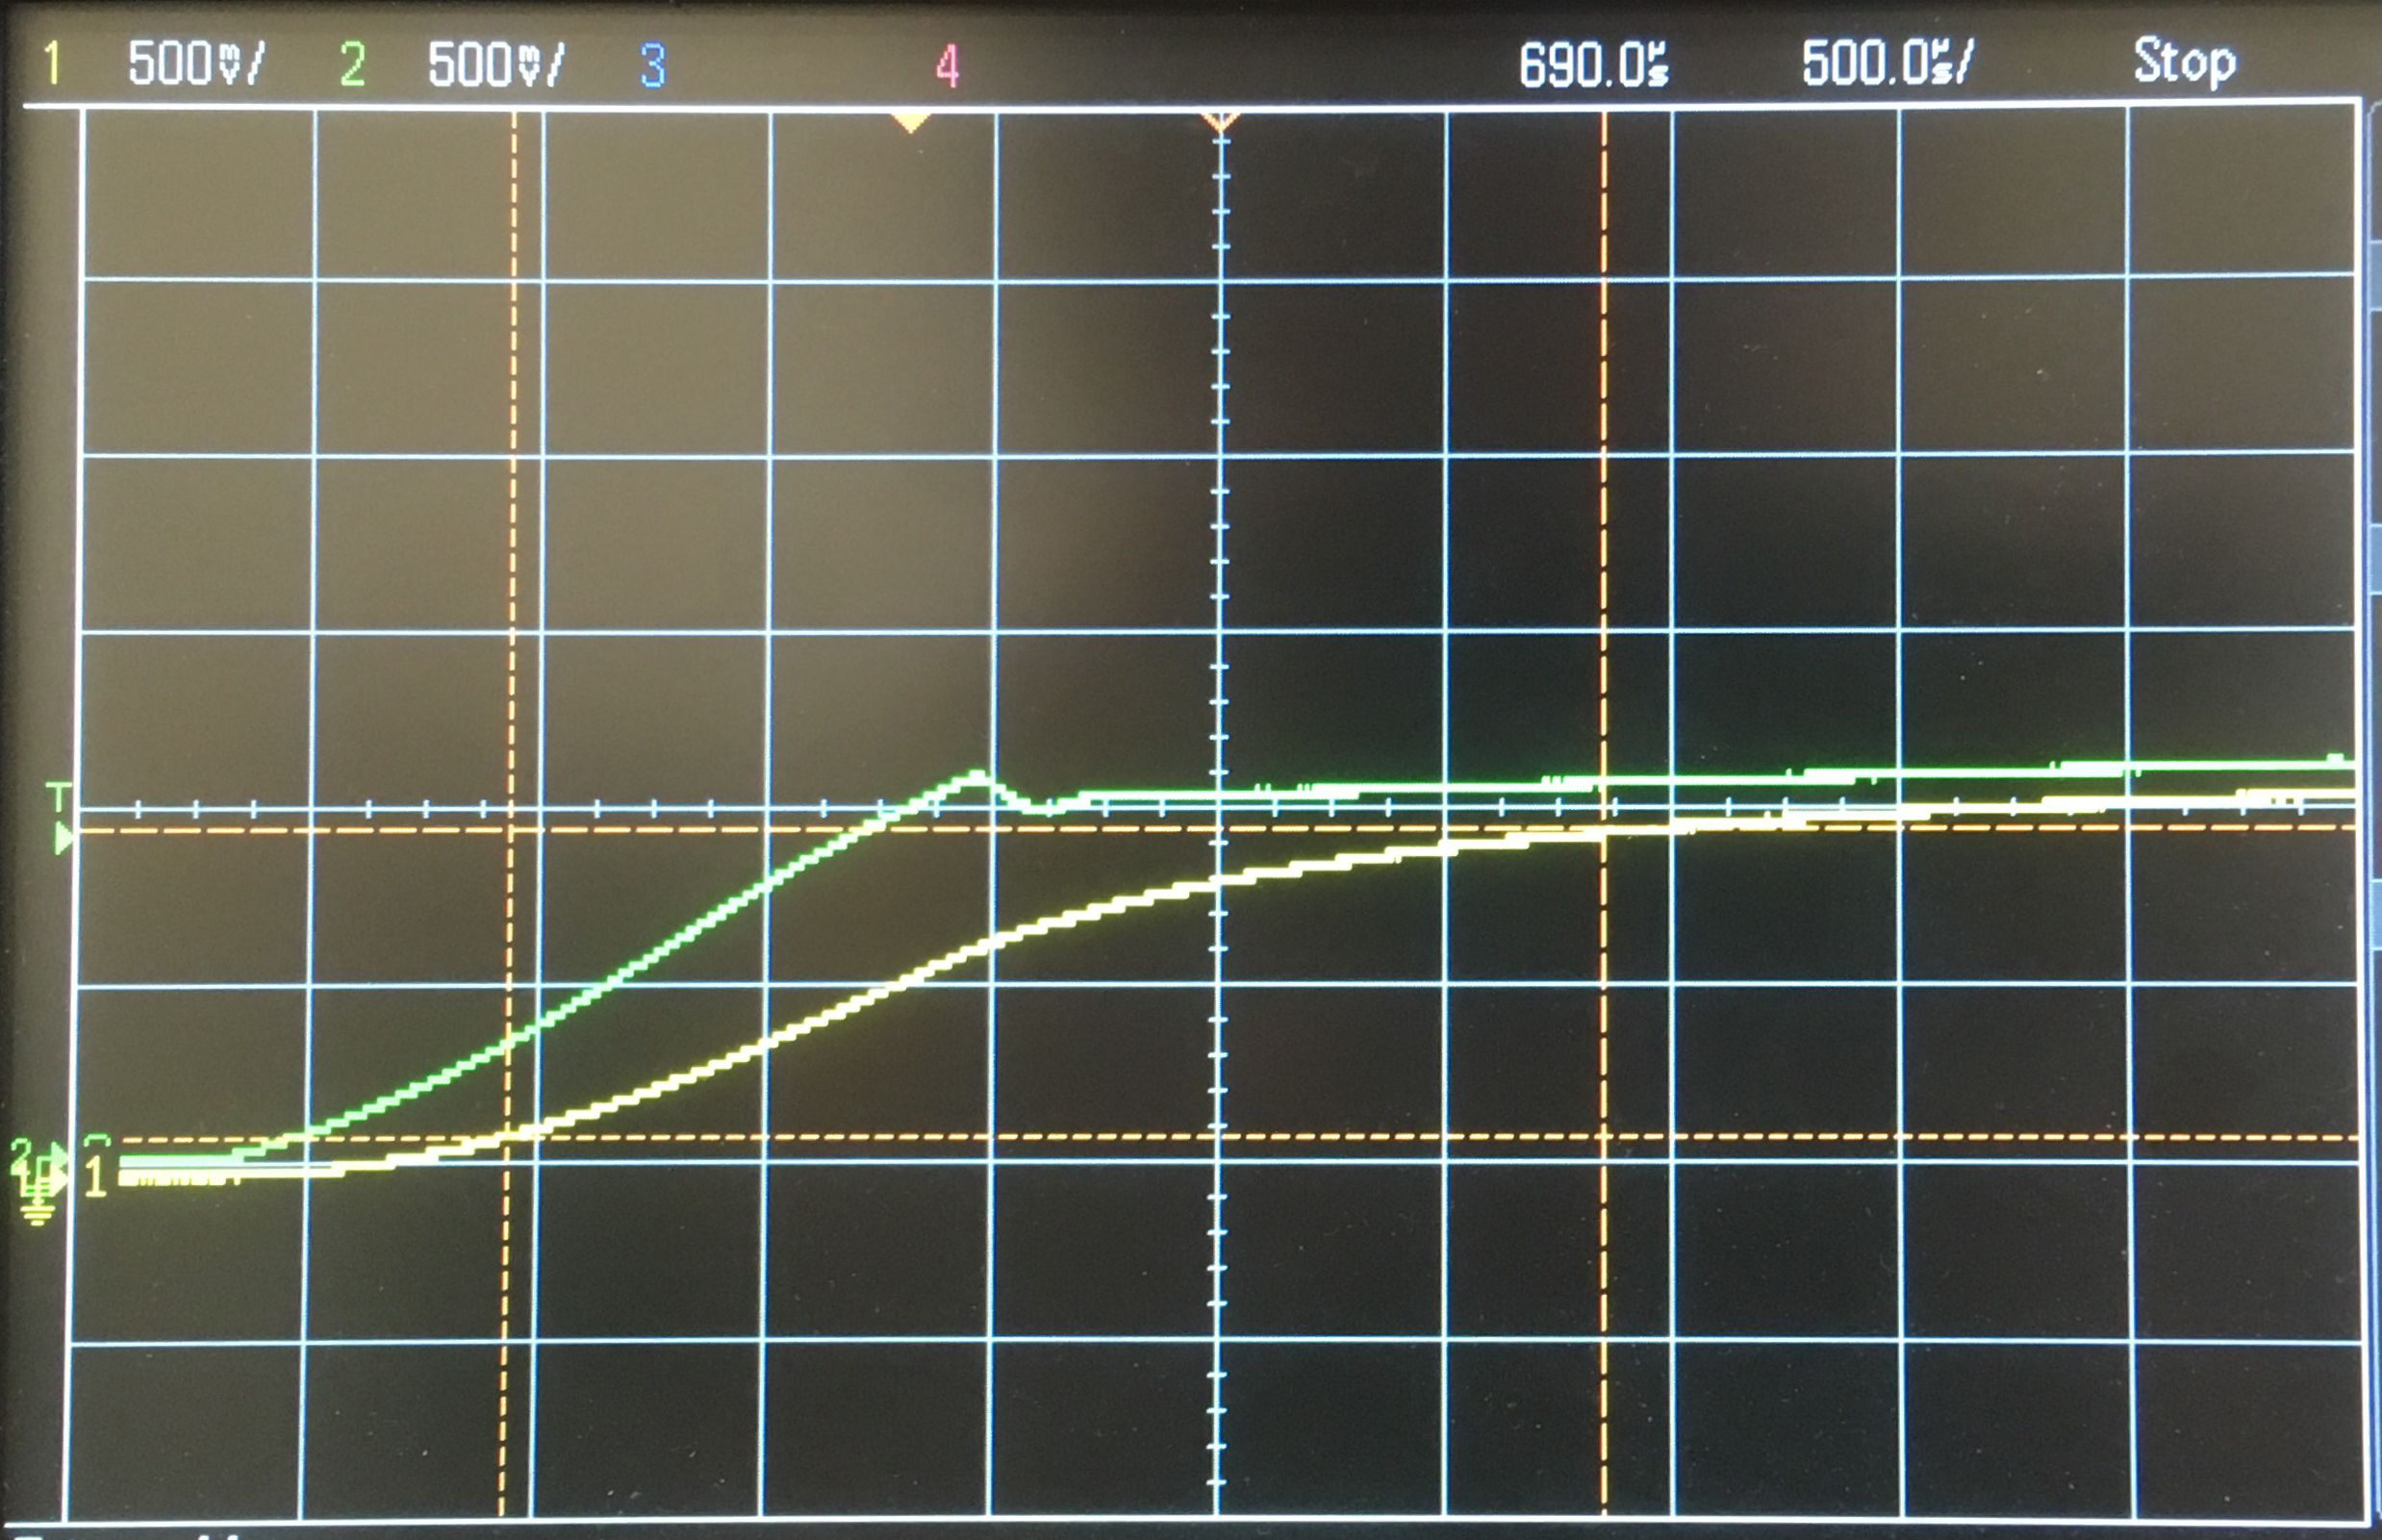
\includegraphics[width=\linewidth]
                {./res/power_on_reset/power_on_reset-zoom.jpg}
        };
        \draw (zoom1.south west) rectangle (zoom1.north east);
    \end{tikzpicture}
    \caption{}
    \end{subfigure}
    \caption[Power-on vs. reset]{
        Both channels have very similar time constant.
        Sorensen XT-76 was used to supply \SI{1.5}{\volt}.
        The green curve was measured on the PSU output.
        This might be the issue that causes unstable power-up.
        Measured on 012.
    }
\end{figure}

Later, we realized that the Rigol, which has a slightly faster time constant,
and can turn on all channels at once, can combine 2 channels so that it can
supply current up to \SI{6}{\ampere}. We changed to the oldest board, and redid
the measurement.

It is worth noting that prior to this measurement, we did not use differential
probes---this was probably a bad idea, and we switched to an oscilloscope with
differential probes to do the measurement this time.

\begin{figure}[ht]
    \centering
    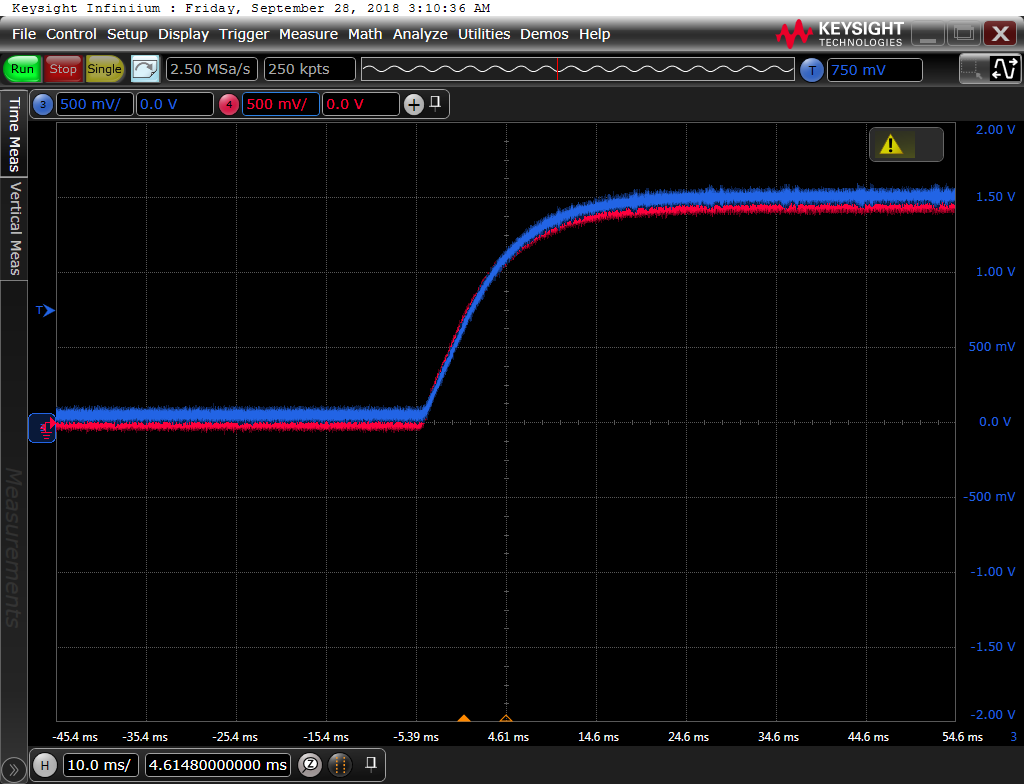
\includegraphics[width=0.8\linewidth]
        {./res/power_on_reset/power_on_reset-008.png}
    \caption[Power-on vs. reset, oldest board]{
        Both channels still have very similar time constant.
        This suggests that DCB has a smaller intrinsic time constant.
        Rigol was used to supply \SI{1.5}{\volt}.
        The green curve was measured on the board.
        After the switch, this board has a higher success (being in state 5)
        rate of power-up.
        Measured on 008.
    }
\end{figure}


\end{document}
